\subsection{用属于函数格的函数逼近连续函数}

在本节中，我们将研究集 \(\mathcal{C} = \mathcal{C}(\mathbf{X};\mathbf{R})\) ，即定义在一个紧空间 \(\mathbf{X}\) 上的连续实值函数(*)全体所成之集，并且总假定 \(\mathcal{C}\) 赋有一致收敛拓扑。由 § 3 第 2 号可知，这个拓扑由范数

\[
| | f | | = \sup _ {x \in \mathbf {X}} | f (x) |
\]

定义，并且这个范数与 C 的 R-代数结构相容。赋有这个范数和这个代数结构的 C 是 R 上的一个完备赋范代数（§ 1 第 6 号，定理 2，推论 1）。

若 H 是 C 的子集，我们称 X 上的连续实值函数 f 可用 H 中的函数一致逼近，如果 f 属于 H 在空间 C 中的闭包，即如果对每个 \(\varepsilon > 0\) ，存在函数 \(g \in H\) ，使得 \(|f(x) - g(x)| \leqslant \varepsilon\) 对一切 \(x \in X\) 成立。因此，说 X 上的每个连续实值函数都可用 H 中的函数一致逼近，就等于说 H 在 C 中稠密。

在集 \(\mathcal{C}\) 上，关系 \(f \leqslant g\) {[}意思是 \(f(x) \leqslant g(x)\) 对一切 \(x \in \mathbf{X}\) 成立{]}是一个序关系，\(\mathcal{C}\) 关于它是一个格。显然有 \(|||u| - |v|| \leqslant ||u - v||\) ，因而 \(u \to |u|\) 是 \(\mathcal{C}\) 到其自身的一致连续映射。由此推出

\[
(u, v) \rightarrow \sup (u, v) = \frac {1}{2} (u + v + | u - v |)
\]

与

\[
(u, v) \rightarrow \inf (u, v) = \frac {1}{2} (u + v - | u - v |)
\]

在 \(\mathcal{C} \times \mathcal{C}\) 上是一致连续的。

命题 1. 设 X 是紧空间，H 是定义在 X 上的连续实值函数所成之集。设 f 是 X 上的连续实值函数，使得对每个 \(x \in X\) 存在函数 \(u_x \in H\) 满足 \(u_x(x) > f(x)\) {[}相应地 \(u_x(x) < f(x)\) {]}。则存在有限个函数 \(u_{x_i} = f_i \in H\) ( \(1 \leqslant i \leqslant n\) )，使得若 \(v = \sup(f_1, f_2, \ldots, f_n)\) {[}相应地 \(w = \inf(f_1, f_2, \ldots, f_n)\) {]}，就有 \(v(x) > f(x)\) {[}相应地 \(w(x) < f(x)\) {]}对一切 \(x \in X\) 成立。

对每个 \(x \in \mathbf{X}\) ，设 \(\mathbf{G}_x\) 是由 \(z \in \mathbf{X}\) 中使 \(u_x(z) > f(z)\) {[}相应地 \(u_x(z) < f(z)\) {]}的 z 全体所组成的开集。由假设 \(x \in \mathbf{G}_x\) ，故 \(\mathbf{X}\) 是诸集 \(\mathbf{G}_x\) (当 \(x\) 跑遍 \(\mathbf{X}\) )的并。由于 \(\mathbf{X}\) 紧，存在有限个点 \(x_i (1 \leqslant i \leqslant n)\) 使得诸 \(\mathbf{G}_{x_i}\) 覆盖 \(\mathbf{X}\) ，并且显然诸函数 \(f_i = u_{x_i}\) 满足命题的条件。

定理 1（迪尼）. 设 X 是紧空间，H 是 X 上的连续实值函数所成之集，它关于关系 \(\leqslant (\text{resp.} \geqslant)\) 是有向的。若 H 的上（相应地，下）包络 f 在 X 上有限且连续，则 f 可用属于 H 的函数一致逼近（或者等价地说，H 的截面滤子在 X 上一致收敛于 f）。

给定 \(\varepsilon > 0\) ，对每个 \(x \in \mathbf{X}\) 存在函数 \(u_x \in \mathbf{H}\) 使得 \(u_x(x) > f(x) - \varepsilon\) 。由命题 1 以及 H 关于关系 \(\leqslant\) 有向这一事实，存在 \(g \in \mathbf{H}\) 使得 \(g(x) > f(x) - \varepsilon\) 对一切 \(x \in \mathbf{X}\) 成立；另一方面，由定义有 \(g(x) \leqslant f(x)\) ，于是定理得证。

推论. 设 \((u_{n})\) 是 X 上连续实值函数的递增（相应地，递减）序列。若序列 \((u_{n})\) 的上（相应地，下）包络 f 在 X 上有限且连续，则序列 \((u_{n})\) 在 X 上一致收敛于 f。

显然，若不再假设 X 紧，定理 1 的结论便未必成立，函数 \(x/(n+x)\) 在 \(R_{+}\) 中的递减序列这一例子便表明了这一点。

命题 2. 设 X 是紧空间，H 是 X 上的连续实值函数所成之集，使得对任意两个函数 \(u \in H\) 、 \(v \in H\) ，函数 \(\sup(u, v)\) 与 \(\inf(u, v)\) 都属于 H。则 X 上的连续实值函数 \(f\) 可用属于 H 的函数一致逼近的充分必要条件是：对每个实数 \(\varepsilon > 0\) 与 X 的每一对点 \(x, y\) ，存在函数 \(u_{x,y} \in H\) ，使得 \(|f(x) - u_{x,y}(x)| < \varepsilon\) 且 \(|f(y) - u_{x,y}(y)| < \varepsilon\) 。

条件显然是必要的；我们来证明它是充分的。对每个 \(\varepsilon > 0\) ，我们将证明存在函数 \(g \in \mathbf{H}\) ，使得 \(|f(z) - g(z)| < \varepsilon\) 对一切 \(z \in \mathbf{X}\) 成立。设 \(x\) 是 \(\mathbf{X}\) 的任意一点，并设 \(\mathbf{H}_x\) 是由函数 \(u \in \mathbf{H}\) (满足 \(u(x) < f(x) + \varepsilon\) )全体所组成之集。由假设，对每个 \(y \in \mathbf{X}\) ，函数 \(u_{x,y}\) 属于 \(\mathbf{H}_x\) 且 \(u_{x,y}(y) > f(y) - \varepsilon\) 。于是由命题 1，存在 \(\mathbf{H}_x\) 中有限个函数，它们的上包络 \(v_x\) 满足 \(v_x(z) > f(z) - \varepsilon\) 对一切 \(z \in \mathbf{X}\) 成立；另一方面，有 \(v_x(x) < f(x) + \varepsilon\) ，这由 \(\mathbf{H}_x\) 的定义得出；最后，由假设 \(v_x \in \mathbf{H}\) 。因此命题 1 表明，存在有限个函数 \(v_{x_i}\) ，它们的下包络 \(g\) 满足 \(g(z) < f(z) + \varepsilon\) 对一切 \(z \in \mathbf{X}\) 成立；但由于 \(v_{x_i}(z) > f(z) - \varepsilon\) 对一切 \(z \in \mathbf{X}\) 及每个指标 \(i\) 成立，故也有 \(g(z) > f(z) - \varepsilon\) 对一切 \(z \in \mathbf{X}\) 成立。由假设 \(g \in \mathbf{H}\) ，证明完毕。

\pandocbounded{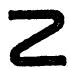
\includegraphics[keepaspectratio]{images/part002_45bf5402.jpg}}

注. 当集 H 满足命题 2 的条件时，它关于序 \(f \leqslant g\) 是一个格。但应指出，C 的子集 H 可以关于这个序是一个格，而 H 中两个函数 u、v 在 H 中的上确界（相应地，下确界）未必与它们在 C 中的上确界（相应地，下确界）相同。* R 的紧区间到 R 中的凸映射提供了一个例子。*

推论. 假设 H 满足：每当 \(u \in H\) 且 \(v \in H\) 时，有 sup \((u, v) \in H\) 与 inf \((u, v) \in H\) ；并且满足：对 X 的任意两个不同点 x、y 与任意两个实数 \(\alpha, \beta\) ，存在函数 \(g \in H\) 使得 \(g(x) = \alpha\) 且 \(g(y) = \beta\) 。则 X 上的每个连续实值函数都可用属于 H 的函数一致逼近。

定义 1. 若 X 是任意集合，X 到集合 Y 中的映射所成之集 H 称为分离 X 的子集 A 的元素（或称为 A 的元素的一个分离集），如果对 A 的任意两个不同元素 x、y，存在函数 \(f \in H\) 使得 \(f(x) \neq f(y)\) 。

例如，若 X 是完全正则空间（第 IX 章，§ 1，第 5 号），则 X 到 {[}0, 1{]} 中的全体连续映射所成之集分离 X 的点。

定理 2（斯通）. 设 X 是紧空间，H 是 C(X; R) 的向量子空间，使得 1) 常数函数属于 H；2) 若 \(u \in H\) ，则 \(|u| \in H\) ；3) H 分离 X 的点。则 X 上的每个连续实值函数都可用 H 中的函数一致逼近。

只需证明 H 满足命题 2 的推论的条件。由假设，若 \(u \in H\) 且 \(v \in H\) ，则有

\[
\sup (u, v) = \frac {1}{2} (u + v + | u - v |) \in H
\]

与

\[
\inf (u, v) = \frac {1}{2} (u + v - | u - v |) \in H.
\]

另一方面，设 \(x\) 与 \(y\) 是 \(X\) 的任意两个不同点，并设 \(\alpha, \beta\) 是任意两个实数。由假设，存在函数 \(h \in H\) 使得 \(h(x) \neq h(y)\) ：设 \(h(x) = \gamma\) ，\(h(y) = \delta\) 。由于常数属于 \(H\) ，函数

\[
g (z) = \alpha + (\beta - \alpha) \frac {h (z) - \gamma}{\delta - \gamma}
\]

属于 H 并且满足 \(g(x) = \alpha\) 与 \(g(y) = \beta\) 。

\subsection{用多项式逼近连续函数}

给定定义在集合 X 上的实值函数所成之集 H，我们称定义在 X 上的实值函数是 H 中函数的实系数多项式（相应地，无常数项的实系数多项式），如果它形如 \(x \to g(f_{1}(x), f_{2}(x), \ldots, f_{n}(x))\) ，其中 g 是 n 个未定元（n 任意）的实系数多项式（相应地，无常数项的多项式），且 \(f_{i}\) ( \(1 \leqslant i \leqslant n\) )属于 H。

定理 3（魏尔斯特拉斯–斯通）. 设 X 是紧空间，H 是 X 上分离 X 的点的连续实值函数所成之集。则 X 上的每个连续实值函数都可用 H 中函数的（实系数）多项式一致逼近。

这个定理的一个等价陈述是：\(\mathcal{C}(\mathbf{X};\mathbf{R})\) 的任一包含常数函数且分离 \(\mathbf{X}\) 的点的子代数在 \(\mathcal{C}(\mathbf{X};\mathbf{R})\) 中稠密。

设 \(H_{0}\) 是 H 中函数的多项式全体所成之集，并设 \(\overline{H}_{0}\) 是 \(H_{0}\) 在 C 中的闭包。若 g 是 n 个变量的任一实系数多项式，则 \((u_{1}, u_{2}, \ldots, u_{n}) \to g(u_{1}, u_{2}, \ldots, u_{n})\) 是 \(C^{n}\) 到 C 中的连续映射，它把 \(H_{0}^{n}\) 映入 \(H_{0}\) ，从而把 \(\overline{H}_{0}^{n}\) 映入 \(\overline{H}_{0}\) （第 I 章，§ 2，第 1 号，定理 1）。特别地，\(\overline{H}_{0}\) 是 C 的向量子空间，并且显然满足定理 2 的第一个与第三个条件；我们将证明它也满足第二个条件，这就证明了 \(\overline{H}_{0} = C\) 。

由于每个函数 \(u \in \overline{\mathbf{H}}_0\) 在 \(\mathbf{X}\) 上有界，只需证明下面的引理：

引理 1. 对每个实数 \(\varepsilon > 0\) 与每个紧区间 \(\mathbf{I} \subset \mathbf{R}\) ，存在无常数项的多项式 \(p(t)\) 使得 \(|p(t) - |t|| \leqslant \varepsilon\) 对一切 \(t \in \mathbf{I}\) 成立。

只需对形如 \(\mathbf{I} = [-a, +a]\) 的区间证明引理，从而（把 \(t\) 换成 \(at\) ）只需对区间 \(\mathbf{I} = [-1, +1]\) 证明。由于 \(|t| = \sqrt{t^2}\) ，引理 1 是下列结果的推论：

引理 2. 设 \((P_n)\) 是由下式定义的无常数项多项式的序列

\[
p _ {0} (t) = 0, \quad p _ {n + 1} (t) = p _ {n} (t) + \frac {1}{2} (t - (p _ {n} (t)) ^ {2}), \quad n \geqslant 0.\tag{1}
\]

在区间 {[}0, 1{]} 中，序列 \((p_n)\) 递增且一致收敛于 \(\sqrt{t}\) 。

为证明引理 2，只需证明对一切 \(t \in [0, 1]\) 有

\[
0 \leqslant \sqrt {t} - p _ {n} (t) \leqslant \frac {2 \sqrt {t}}{2 + n \sqrt {t}},\tag{2}
\]

因为 (2) 蕴涵 \(0 \leqslant \sqrt{t} - p_n(t) \leqslant 2 / n\) 。

我们对 \(n\) 用归纳法证明 (2) 。它对 \(n = 0\) 成立。若 \(n \geqslant 0\) ，由归纳假设 (2) 得 \(0 \leqslant \sqrt{t} - p_n(t) \leqslant \sqrt{t}\) ，从而 \(0 \leqslant p_n(t) \leqslant \sqrt{t}\) ，于是由 (1) 有

\[
\sqrt {t} - p _ {n + 1} (t) = (\sqrt {t} - p _ {n} (t)) \left(1 - \frac {1}{2} (\sqrt {t} + p _ {n} (t))\right),
\]

因而 \(\sqrt{t} - p_{n+1}(t) \geqslant 0\) ，并且由 (2)

\[
\begin{array}{r l} \sqrt {t} - p _ {n + 1} (t) & \leqslant \frac {2 \sqrt {t}}{2 + n \sqrt {t}} \left(1 - \frac {\sqrt {t}}{2}\right) \leqslant \frac {2 \sqrt {t}}{2 + n \sqrt {t}} \left(1 - \frac {\sqrt {t}}{2 + (n + 1) \sqrt {t}}\right) \\ & = \frac {2 \sqrt {t}}{2 + (n + 1) \sqrt {t}}. \end{array} \tag {Q.E.D.}
\]

若 X 不紧，定理 3 的结论未必成立。例如，R 上有界且非常数的连续实值函数不能在 R 中用多项式一致逼近（参见习题 6）。

命题 3. 设 \((\mathbf{K}_t)_{t \in \mathbf{I}}\) 是 \(\mathbf{R}\) 的紧区间的一个族，\(\mathbf{K} = \prod_{t \in \mathbf{I}} \mathbf{K}_t\) 是它们的乘积，并设 \(\mathbf{X}\) 是 \(\mathbf{K}\) 的一个紧子空间。则 \(\mathbf{X}\) 上的每个连续实值函数都可用坐标 \(x_t = \mathrm{pr}_t x\) 的多项式一致逼近。

因为若 \(x = (x_{t})\) 与 \(y = (y_{t})\) 是 X 的两个不同点，则至少存在一个指标 t 使得 \(x_{t} \neq y_{t}\) ；因而连续函数族 \(pr_{t}\) 满足定理 3 的条件。

命题 4. 设 X 是紧空间，A 是 X 的闭子空间，H 是 X 上分离 \(\mathbb{C}A\) 的点的连续实值函数所成之集，并且当 u 跑遍 H 时，A 是诸集 \(\overline{u}^{1}(0)\) 的交。则 X 上在 A 上为零的每个连续实值函数都可用 H 中函数的无常数项多项式一致逼近。

先考虑 A 仅由一点 \(x_{0}\) 组成的特殊情形。这时诸假设蕴涵 H 分离 X 的点；因为若 \(x \neq x_{0}\) ，则由假设存在函数 \(u \in H\) 使得 \(u(x) \neq 0 = u(x_{0})\) 。于是，对每个 \(\varepsilon > 0\) 与每个满足 \(f(x_{0}) = 0\) 的 X 上的连续实值函数 f，存在（定理 3）H 中函数的一个多项式 g，使得 \(|f(x) - g(x)| \leqslant \varepsilon\) 对一切 \(x \in X\) 成立。特别地 \(|g(x_{0})| \leqslant \varepsilon\) ，从而

\[
\left| f (x) - \left(g (x) - g \left(x _ {0}\right)\right) \right| \leqslant 2 \varepsilon
\]

对一切 \(x \in \mathbf{X}\) 成立；又由于 \(g(x) - g(x_0)\) 是 \(\mathbf{H}\) 中函数的一个无常数项多项式，该情形的结论得证。

在一般情形，考察 X 上的等价关系 R，它的类是集合 A 与诸集 \(\{x\}\) ( \(x \notin A\) )。商空间 X/R 是豪斯多夫的（第 I 章，§ 8，第 6 号，命题 15），从而是紧的。设 \(\varphi: X \to X/R\) 是典范映射。X 上每个在 A 上为零的连续实值函数 f 都可写成 \(f = f_{1} \circ \varphi\) 的形式，其中 \(f_{1}\) 是 X/R 上在点 \(x_{0}' = \varphi(A)\) 处为零的连续实值函数。把已证的结果应用于空间 X/R 与点 \(x_{0}'\) ，即得最终结论。

\subsection{应用：定义在紧空间的乘积上的连续实值函数的逼近}

定理 4. 设 \((\mathbf{X}_t)_{t\in \mathbf{I}}\) 是紧空间的一个族，并令

\[
\mathrm{X} = \prod_ {t \in \mathrm{I}} \mathrm{X} _ {t}.
\]

则 X 上的每个连续实值函数都可用有限多个下列形式的函数之和一致逼近：

\[
(x _ {t}) \rightarrow \prod_ {\alpha \in \mathbf {J}} u _ {\alpha} (x _ {\alpha}),
\]

其中 J 是 I 的（任意）有限子集，而 \(u_{\alpha}\) 是 \(X_{\alpha}\) 上的连续实值函数（对每个 \(\alpha \in J\) ）。

考察 H，即在 X 上连续的“单元函数” \((x_{t}) \rightarrow u_{\alpha}(x_{\alpha})\) (任意 \(\alpha \in I\) )所成的集。这个集分离 X 的点，因为若 \(x = (x_{t})\) 与 \(y = (y_{t})\) 是 X 的任意两个不同点，则存在 \(\alpha \in I\) 使 \(x_{\alpha} \neq y_{\alpha}\) ，并且存在连续实值函数 \(h_{\alpha}\) ，它定义在 \(X_{\alpha}\) 上且使 \(h_{\alpha}(x_{\alpha}) \neq h_{\alpha}(y_{\alpha})\) 。于是函数 \(x \rightarrow h_{\alpha}(\operatorname{pr}_{\alpha} x)\) 属于 H 且在 x 与 y 处取不同的值。由于 H 中函数的每个多项式都具有定理中所述的形式，结论由定理 3 得出。

若诸 \(X_{t}\) 并非全为紧的，定理 4 的结论未必成立（参见习题 9）。

\subsection{紧空间到赋范空间中的连续映射的逼近}

设 X 是紧空间，Y 是域 R 上的赋范向量空间（第 IX 章，§ 3）；我们总假定空间 \(\mathcal{C}(\mathbf{X};\mathbf{Y})\) 赋有由范数 \(||u|| = \sup_{x\in \mathbf{X}}||u(x)||\) 定义的一致收敛拓扑（§ 3，第 2 号）。

给定连续实值函数所成的一个集 \(\mathbf{H}\) (这些函数定义在 \(\mathbf{X}\) 上)、函数的一个有限族 \((u_i)_{1\leqslant i\leqslant n}\) (属于 \(\mathbf{H}\) )以及点的一个有限族 \((a_i)_{1\leqslant i\leqslant n}\) (属于 \(\mathbf{Y}\) )：映射 \(x\to \sum_{i = 1}^{n}a_iu_i(x)\) 是 \(\mathbf{X}\) 到 \(\mathbf{Y}\) 中的连续映射；我们把它记作 \(\sum_{i = 1}^{n}a_iu_i\) ，并称它为 \(\mathbf{H}\) 中函数的以 \(\mathbf{Y}\) 中元素为系数的线性组合。我们说连续映射 \(f:\mathbf{X}\rightarrow \mathbf{Y}\) 可用 \(\mathbf{H}\) 中函数的线性组合（以 \(\mathbf{Y}\) 中元素为系数）一致逼近，如果 \(f\) 属于由这些线性组合构成的 \(\mathcal{C}(\mathbf{X};\mathbf{Y})\) 的向量子空间的闭包。

命题 5. 设 X 是紧空间，Y 是 R 上的赋范空间，H 是 C (X; R) 的一个子集。若 X 上每个连续实值函数都可用 H 中函数一致逼近，则每个 X 到 Y 中的连续映射 f 都可用 H 中函数的以 Y 中元素为系数的线性组合一致逼近。

给定任意实数 \(\varepsilon > 0\) ，对每个 \(x \in \mathbf{X}\) ，存在 \(x\) 的一个开邻域，\(f\) 在其中的振幅 \(\leqslant \varepsilon\) 。因而存在一个有限开覆盖 \((\mathrm{A}_i)_{1 \leqslant i \leqslant n}\) (它覆盖 \(\mathbf{X}\) )，使得 \(f\) 在每个 \(\mathrm{A}_i\) 中的振幅 \(\leqslant \varepsilon\) 。设 \(\boldsymbol{a}_i\) 是 \(f\) 在 \(\mathrm{A}_i\) 中的一个值 ( \(1 \leqslant i \leqslant n\) )，并设 \((u_i)_{1 \leqslant i \leqslant n}\) 是从属于覆盖 \((\mathrm{A}_i)\) 的连续单位分解（第 IX 章，§ 4，第 4 号，命题 4 的推论）。设 \(x\) 是 \(\mathbf{X}\) 的任意一点。对每个指标 \(i\) (满足 \(x \notin \mathrm{A}_i\) )，有 \(u_i(x) = 0\) ，而对每个指标 \(i\) (满足 \(x \in \mathrm{A}_i\) )，有 \(||f(x) - a_i|| \leqslant \varepsilon\) ；由此得出

\[
\left\| \boldsymbol {f} (x) - \sum_ {i = 1} ^ {n} \boldsymbol {a} _ {i} u _ {i} (x) \right\| = \left\| \sum_ {i = 1} ^ {n} (\boldsymbol {f} (x) - \boldsymbol {a} _ {i}) u _ {i} (x) \right\| \leqslant \varepsilon \sum_ {i = 1} ^ {n} u _ {i} (x) = \varepsilon .
\]

另一方面，由假设存在函数 \(v_{i} \in \mathbf{H}\) 使得

\[
\left| u _ {i} (x) - v _ {i} (x) \right| \leqslant \frac {\varepsilon}{\sum_ {j = 1} ^ {n} | | \boldsymbol {a} _ {j} | |}
\]

对一切 \(x \in \mathbf{X} (1 \leqslant i \leqslant n)\) 成立；因而有

\[
\left\| \boldsymbol {f} (x) - \sum_ {i = 1} ^ {n} \boldsymbol {a} _ {i} v _ {i} (x) \right\| \leqslant 2 \varepsilon \text {   for   all   } x \in \mathbf {X},
\]

证毕。

由命题 5 可得：对于我们已证明 C(X; R) 的某个子集 H 为稠密的每个命题，都有一个关于 X 到任意赋范空间 Y 中的连续映射的类似命题与之对应。我们只明确写出以这种方式对应于定理 3 的命题。给定 X 上实值函数所成的一个集 H，H 中函数的以 Y 为系数的多项式定义为属于 H 的函数的一个有限（可以是空的）族的乘积以 Y 中元素为系数的线性组合。于是：

命题 6. 设 X 是紧空间，H 是 X 上分离 X 的点的连续实值函数所成之集。则每个 X 到 R 上的赋范空间 Y 中的连续映射都可用 H 中函数的以 Y 中元素为系数的多项式一致逼近。

由此我们推出：

命题 7. 设 X 是紧空间，H 是 X 上分离 X 的点的连续复值函数所成之集。则每个 X 到 C 上的赋范空间 Y 中的连续映射都可用函数 \(f \in \mathbf{H}\) 及其共轭 \(\overline{f}\) 的以 Y 中元素为系数的多项式一致逼近。

只需注意 Y 也是 R 上的赋范空间，并对函数 \(f \in H\) 的实部与虚部所成的集应用命题 6，利用公式

\[
\mathfrak {R} f = \frac {1}{2} (f + \overline {{f}}), \quad \Im f = \frac {1}{2 i} (f - \overline {{f}}).
\]

推论 1. 若 X 是空间 \(\mathbf{C}^n\) 的紧子集，则每个 X 到域 C 上的赋范空间 Y 中的连续映射 \((z_1, z_2, \ldots, z_n) \to f(z_1, z_2, \ldots, z_n)\) 都可用 \(z_k\) 与 \(\overline{z}_k\) 的以 Y 中元素为系数的多项式一致逼近。

\pandocbounded{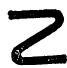
\includegraphics[keepaspectratio]{images/part002_94458643.jpg}}

我们以后将会看到，一般说来，即使 Y = C，也不可能用仅含变量 \(z_{k}\) 的（以 Y 中元素为系数的）多项式一致逼近 f。

推论 2. 设 X 是局部紧空间，\(\mathcal{C}_0(\mathbf{X})\) 是 X 到 C 中的在无穷远处趋于 0 的连续映射所成的赋范 C-代数。设 A 是 \(\mathcal{C}_0(\mathbf{X})\) 的一个分离 X 的点的子代数，且满足：(i) \(\overline{f} \in \mathbf{A}\) ，只要 \(f \in \mathbf{A}\) ；(ii) 对每个 \(x \in \mathbf{X}\) ，存在 \(f \in \mathbf{A}\) 使 \(f(x) \neq 0\) 。则 A 在 \(\mathcal{C}_0(\mathbf{X})\) 中稠密。

若 \(X'\) 是由 X 添加一个无穷远点 \(\omega\) 而得到的紧空间，则 \(\mathcal{C}_{0}(\mathbf{X})\) 可等同于 \(\mathcal{C}(\mathbf{X};\mathbf{C})\) 中由在 \(\omega\) 处为零的连续映射组成的子空间，\(\mathcal{C}_{0}(\mathbf{X})\) 上的范数由下式定义：

\[
\left| \left| f \right| \right| = \sup _ {x \in \mathbf {X}} | f (x) | = \sup _ {x \in \mathbf {X}'} | f (x) |.
\]

根据命题 7，每个 \(f \in \mathcal{C}_{0}(X)\) 都可用 A 中函数的复系数多项式一致逼近；此外，由于 \(f(\omega) = 0\) ，第 2 号命题 4 的论证表明可设这些多项式无常数项，于是它们属于 A。

命题 7 的另一个应用如下：

命题 8. 设 P 是 \(\mathbf{R}^m\) 到 \(\mathbf{C}\) 中的其周期群包含 \(\mathbf{Z}^m\) 的周期连续映射全体所成之集。则属于 P 的每个函数都可在 \(\mathbf{R}^m\) 中用下列形式的函数的复系数线性组合一致逼近：

\[
(x _ {1}, x _ {2}, \dots , x _ {m}) \rightarrow e (h _ {1} x _ {1} + h _ {2} x _ {2} + \dots + h _ {m} x _ {m}),
\]

其中 \(h_{i}\) 是有理整数（这样的线性组合称为 m 个变量的三角多项式）。

只需注意，P（赋有一致收敛拓扑）典范同构于紧空间 \(T^{m}\) 到 C 中的所有连续映射所成的空间（第 VII 章，§ 1，第 6 号），并对 \(T^{m}\) 到 C 中的与 m 个映射 \((x_{1}, x_{2}, \ldots, x_{m}) \to e(x_{i}) \quad (1 \leqslant i \leqslant m)\) (即 \(R^{m}\) 到 C 中的映射)相对应的映射所成之集应用命题 7。

\ExerciseGroupsStart

\ExerciseSection

\begin{enumerate}
\def\labelenumi{\arabic{enumi})}
\tightlist
\item
  设 X 是一个集，Y 是一个含多于一个点的一致空间，S 是 X 的非空子集所成的一个非空集。设 \(Y' \subset \mathcal{F}(X; Y)\) 是 X 到 Y 中的常值映射全体所成之集。对每个 \(y \in Y\) ，设 \(c_{y}\) 是以 y 为值的 X 到 Y 中的常值映射。
\end{enumerate}

\begin{enumerate}
\def\labelenumi{\alph{enumi})}
\item
  证明 \(y \to c_{y}\) 是 Y 到一致子空间 \(Y'\) ( \(\mathcal{F}_{\mathfrak{S}}(\mathbf{X}; \mathbf{Y})\) 的一致子空间)上的一个同构。
\item
  \(\mathcal{F}_{\mathfrak{S}}(\mathbf{X};\mathbf{Y})\) 是豪斯多夫的，当且仅当 Y 是豪斯多夫的且 \(\mathfrak{S}\) 是 X 的一个覆盖。
\item
  \(\mathbf{Y}'\) 在 \(\mathcal{F}_{\mathfrak{S}}(\mathbf{X};\mathbf{Y})\) 中是闭的，当且仅当 \(\mathcal{F}_{\mathfrak{S}}(\mathbf{X};\mathbf{Y})\) 是豪斯多夫的。
\end{enumerate}

\begin{enumerate}
\def\labelenumi{\arabic{enumi})}
\setcounter{enumi}{1}
\tightlist
\item
  设 X 是一个集，Y 是一个含多于一个点的豪斯多夫一致空间，\(\mathfrak{S}_1, \mathfrak{S}_2\) 是 X 的子集所成的两个集，它们满足第 2 号的条件 \((\mathrm{F}_{\mathrm{I}}^{\prime}), (\mathrm{F}_{\mathrm{II}}^{\prime})\) 。证明若 \(\mathfrak{S}_1 \subset \mathfrak{S}_2\) 且 \(\mathfrak{S}_1 \neq \mathfrak{S}_2\) ，则 \(\mathfrak{S}_1\) -收敛的一致结构严格粗于 \(\mathfrak{S}_2\) -收敛的一致结构。特别地：
\end{enumerate}

\begin{enumerate}
\def\labelenumi{(\roman{enumi})}
\item
  若 X 是非紧的豪斯多夫拓扑空间，则紧收敛的一致结构严格粗于一致收敛的一致结构。
\item
  若 X 是具有无限紧子集的豪斯多夫拓扑空间（参见第 I 章，§ 9，习题 4），则逐点收敛的一致结构严格粗于紧收敛的一致结构。
\end{enumerate}

\begin{enumerate}
\def\labelenumi{\arabic{enumi})}
\setcounter{enumi}{2}
\item
  设 X 是一个集，S 是 X 的一个覆盖，Y 是一个非豪斯多夫的一致空间，\(Y_{0}\) 是与 Y 相伴的豪斯多夫一致空间（第 II 章，§ 3，第 8 号）。证明与 \(\mathcal{F}_{\mathfrak{S}}(\mathrm{X};\mathrm{Y})\) 相伴的豪斯多夫一致空间同构于 \(\mathcal{F}_{\mathfrak{S}}(\mathrm{X};\mathrm{Y}_{0})\) 。
\item
  证明在集 \(\mathcal{C}(\mathbf{R};\mathbf{R})\) (即定义在 \(\mathbf{R}\) 上的有限连续实值函数全体所成之集)上，关于 R 的加法一致结构的一致收敛拓扑不同于关于由扩充实直线 \(\overline{R}\) 的（唯一的）一致结构在 R 上诱导的一致结构的一致收敛拓扑（尽管这两个一致结构在 R 上诱导的拓扑相同）。
\item
  设 X 是拓扑空间。X 的子集所成的集 S 称为饱和的，如果它满足第 2 号的条件 \((\mathbf{F}_{\mathbf{I}}^{\prime})\) 与 \((\mathbf{F}_{\mathbf{II}}^{\prime})\) ，并且 S 中每个集的闭包属于 S。
\end{enumerate}

\begin{enumerate}
\def\labelenumi{\alph{enumi})}
\item
  证明若 X 是正规的且 S 是饱和的并覆盖 X，则集 C(X; R) 在空间 \(\tilde{\mathcal{C}}_{\mathfrak{S}}(X; \mathbf{R})\) (第 6 号，定理 2，推论 2)中关于 S-收敛拓扑是稠密的。特别地，C(X; R) 在 \(F_{s}(X; \mathbf{R})\) 中稠密。只有当 X 是离散的时，C(X; R) 才在 \(F_{s}(X; \mathbf{R})\) 中是闭的。
\item
  设 X 是完全正则空间（第 IX 章，§ 1，第 5 号），\(\mathfrak{S}_1, \mathfrak{S}_2\) 是 X 的子集所成的两个饱和集，满足 \(\mathfrak{S}_1 \subset \mathfrak{S}_2\) 且 \(\mathfrak{S}_1 \neq \mathfrak{S}_2\) 。证明 \(\mathfrak{S}_1\) -收敛在 \(\mathcal{C}(\mathbf{X}; \mathbf{R})\) 上的拓扑严格粗于 \(\mathfrak{S}_2\) -收敛的拓扑。
\end{enumerate}

\begin{enumerate}
\def\labelenumi{\arabic{enumi})}
\setcounter{enumi}{5}
\tightlist
\item
  \begin{enumerate}
  \def\labelenumii{\alph{enumii})}
  \tightlist
  \item
    设 X 是拓扑空间，Y 是一致空间，\(\Phi\) 是 \(\mathcal{C}(X;Y)\) 所成之集上逐点收敛于函数 \(u_{0}\) 的一个滤子。则 \(u_{0}\) 在一点 \(x_{0}\in X\) 处连续，当且仅当对 Y 的每个围域 V 与每个集 \(M\in\Phi\) ，存在 \(x_{0}\) 的一个邻域 U 与一个映射 \(u\in M\) ，使得 \((u_{0}(x),u(x))\in V\) 对一切 \(x\in U\) 成立。
  \end{enumerate}
\end{enumerate}

\begin{enumerate}
\def\labelenumi{\alph{enumi})}
\setcounter{enumi}{1}
\tightlist
\item
  设 X 是拟紧空间，Y 是一致空间，\(\Phi\) 是 \(\mathcal{C}(X;Y)\) 上逐点收敛于函数 \(u_{0}\) 的一个滤子。则 \(u_{0}\) 在 X 上连续，当且仅当对 Y 的每个围域 V 与每个集 \(M\in\Phi\) ，存在有限个函数 \(u_{i}\in\mathbf{M}(1\leqslant i\leqslant n)\) ，使得对每个 \(x\in X\) ，至少对一个指标 i 有 \((u_{0}(x),u_{i}(x))\in V\) 。
\end{enumerate}

\begin{enumerate}
\def\labelenumi{\arabic{enumi})}
\setcounter{enumi}{6}
\tightlist
\item
  设 X、Y 是两个豪斯多夫一致空间。对每个连续映射 \(f: \mathbf{X} \to \mathbf{Y}\) ，设 \(\mathbf{G}(f) \subset \mathbf{X} \times \mathbf{Y}\) 是 \(f\) 的图象；\(\mathbf{G}(f)\) 在 \(\mathbf{X} \times \mathbf{Y}\) 中是闭的（第 I 章，§ 8，第 1 号，命题 2，推论 2）：因而 \(f \to \mathbf{G}(f)\) 是 \(\mathcal{C}(\mathbf{X}; \mathbf{Y})\) 到 \(\mathfrak{F}(\mathbf{X} \times \mathbf{Y})\) (即 \(\mathbf{X} \times \mathbf{Y}\) 的非空闭子集全体所成之集)中的一个单射映射。
\end{enumerate}

\begin{enumerate}
\def\labelenumi{\alph{enumi})}
\item
  证明映射 \(f \to \mathbf{G}(f)\) (它把 \(\mathcal{C}_u(\mathbf{X};\mathbf{Y})\) 映到 \(\mathfrak{F}(\mathbf{X}\times \mathbf{Y})\) 中)当 \(\mathfrak{F}(\mathbf{X}\times \mathbf{Y})\) 赋有第 II 章，§ 1，习题 5 中定义的一致结构时是一致连续的。
\item
  设 \(\Gamma\) 是 \(\mathcal{C}(\mathbf{X};\mathbf{Y})\) 在 \(\mathfrak{F}(\mathbf{X}\times \mathbf{Y})\) 中 (在映射 \(f\to \mathbf{G}(f)\) 下)的象，并设 \(\varphi :\Gamma \to \mathcal{C}_u(\mathbf{X};\mathbf{Y})\) 是逆映射。证明若 \(\mathbf{X}\) 紧，则 \(\varphi\) 在 \(\Gamma\) 上连续（用反证法论证）。
\item
  取 X 与 Y 都为 R 的紧区间 {[}0, 1{]} 。证明 \(\varphi\) 在 \(\Gamma\) 上不是一致连续的。
\end{enumerate}

\begin{enumerate}
\def\labelenumi{\arabic{enumi})}
\setcounter{enumi}{7}
\tightlist
\item
  设 X、Y 是两个度量空间，\((f_{n})\) 是 X 到 Y 中的 \(\alpha\) 类波莱尔映射的一个序列（第 IX 章，§ 6，习题 16）。
\end{enumerate}

\begin{enumerate}
\def\labelenumi{\alph{enumi})}
\item
  假设序列 \((f_{n})\) 逐点收敛于映射 f: X → Y。证明 f 是 \(\alpha + 1\) 类的。{[}若 U 是 Y 的开子集，注意 \(\overline{f}^{1}(U) = \bigcup_{n \geqslant 1} \left( \bigcap_{k \geqslant 0} \overline{f}_{n+k}^{1}(U) \right)\) ，并利用第 IX 章，§ 6，习题 4。{]}
\item
  假设序列 \((f_n)\) 一致收敛于 \(f\) 。证明 \(f\) 是 \(\alpha\) 类的。{[}设 \(\mathbf{F}\) 是 \(\mathbf{Y}\) 的一个闭子集，且对每个整数 \(n > 0\) ，设 \(\mathbf{V}_n\) 是 \(\mathbf{Y}\) 中与 \(\mathbf{F}\) 的距离 \(\leqslant 1/n\) 的点所成之集。证明存在整数的一个递增序列 \(n \to m(n)\) 使得 \(\overline{f}^1(\mathbf{F}) = \bigcap_{n} \overline{f}_{m(n)}^1(\mathbf{V}_n)\) 。{]}
\item
  假设 Y 是可数型的。证明若 \(f: X \to Y\) 是 \(\alpha > 0\) 类的波莱尔函数，则存在波莱尔函数的一个序列 \(g_{n}: X \to Y\) ，它们是 \(<\alpha\) 类的，使得 \((g_{n})\) 逐点收敛于 f。{[}证明可取 \(g_{n}\) 为只取有限多个值的函数；利用第 IX 章，§ 6 的习题 4 h) 与 16 c)。{]}
\end{enumerate}

\begin{enumerate}
\def\labelenumi{\arabic{enumi})}
\setcounter{enumi}{8}
\item
  设 X 是贝尔空间，Y 是度量空间，\((f_{n})\) 是 X 到 Y 中的连续映射的一个序列，它逐点收敛于函数 f。点 \(x \in X\) 称为序列 \((f_{n})\) 的一致收敛点，如果对每个 \(\varepsilon > 0\) ，存在 x 的一个邻域 V 与一个整数 p，使得 \(d(f_{m}(y), f_{n}(y)) \leqslant \varepsilon\) 对一切 \(y \in V\) 与一切整数 \(m \geqslant p, n \geqslant p, d\) 成立，其中 d 是 Y 上的度量。证明序列 \((f_{n})\) 的一致收敛点所成之集的余集 S 在 X 中是贫集{[}参见第 IX 章，§ 5，习题 22 a{]}。给出一个 S 在 X 中稠密的例子。{[}取 X = Y = R，设 \(n \to r_{n}\) 是 N 到 Q 上的一个双射，并设 \((g_{n})\) 是 R 到 {[}0, 1{]} 中的连续映射的一个序列，它对 \(x \neq 0\) 收敛于零函数而在 x = 0 处收敛于 1，且在每个不含 0 的 R 的开集中收敛是一致的。然后考察函数序列 \(f_{n}(x) = \sum_{p=0}^{\infty} \alpha_{p} g_{n}(x - r_{p})\) ，其中序列 \((\alpha_{p})\) 以适当的方式趋于 0。{]}
\item
  证明在群 \(\Gamma\) (由实直线 \(\mathbf{R}\) 到其自身上的同胚组成)上，逐点收敛拓扑与紧收敛拓扑相同（参见 § 3，习题 14）。
\item
  设 X 是拓扑空间，G 是拓扑群。X 到 G 中的连续映射所成之集 C(X; G) 是群 \(G^{X}\) 的一个子群。设 S 是 X 的子集所成的一个集。
\end{enumerate}

\begin{enumerate}
\def\labelenumi{\alph{enumi})}
\item
  假设对每个 \(A \in S\) 、G 中 e 的每个邻域 V 与每个 \(u \in C(X; G)\) ，存在 G 中 e 的一个邻域 W，使得 \(sWs^{-1} \subset W\) 对一切 \(s \in u(A)\) 成立。证明 S-收敛拓扑这时与 \(\mathcal{C}(X; G)\) 的群结构相容，且如此定义的拓扑群 \(\mathcal{C}_{\mathfrak{S}}(X; G)\) 的右（相应地，左）一致结构与 S-收敛的一致结构相同。考察逐点收敛的情形、G 局部紧时紧收敛的情形，以及 G 交换的情形。
\item
  若 G 是群 \(\mathbf{SL}(2, \mathbf{R})\) ，赋有由 \(R^{4}\) 的拓扑诱导的拓扑，证明一致收敛拓扑与 \(\mathcal{C}(\mathbf{R}; \mathbf{G})\) 的群结构不相容。
\end{enumerate}

\begin{enumerate}
\def\labelenumi{\arabic{enumi})}
\setcounter{enumi}{11}
\tightlist
\item
  设 X 是拓扑空间，A 是拓扑环（第 III 章，§ 6，第 3 号）。X 到 A 中的连续映射所成之集 C(X; A) 是环 A\^{}X 的一个子环。设 S 是 X 的子集所成的一个集。
\end{enumerate}

\begin{enumerate}
\def\labelenumi{\alph{enumi})}
\item
  假设对每个 \(\mathbf{M} \in \mathfrak{S}\) 与每个 \(u \in \mathcal{C}(\mathbf{X}; \mathbf{A})\) ，集 \(u(\mathbf{M})\) 是有界的（第 III 章，§ 6，习题 12）。证明 \(\mathfrak{S}\) -收敛拓扑与 \(\mathcal{C}(\mathbf{X}; \mathbf{A})\) 的环结构相容。考察逐点收敛的情形与紧收敛的情形。
\item
  设 X 是一个非紧的局部紧 \(\sigma\) -紧空间（第 I 章，§ 9，第 9 号）。证明一致收敛拓扑与 \(\mathcal{C}\) (X; R) 的环结构不相容。
\end{enumerate}

\ExerciseSection

\begin{enumerate}
\def\labelenumi{\arabic{enumi})}
\item
  设 \(f\) 是 \(\mathbf{R}\) 上的实值函数，它等于 \(0\) （当 \(x \leqslant 0\) ），等于 \(x\) （当 \(0 \leqslant x \leqslant 1\) ），等于 \(1\) （当 \(x \geqslant 1\) ）。证明实值函数序列 \(f_n(x) = f(nx - n^2)\) ( \(n \in \mathbf{N}\) ) 是等度连续的但在 \(\mathbf{R}\) 上不是一致等度连续的，尽管它由一致连续函数组成。
\item
  设 X 是每个点都具有可数基本邻域系的豪斯多夫拓扑空间，Y 是一致空间。设 H 是 \(\mathcal{C}(X;Y)\) 的一个子集，具有下列性质：对 X 的每个紧子集 K，集 \(H|K\) (由映射 \(u\in H\) 在 K 上的限制组成)是 \(\mathcal{C}(K;Y)\) 的一个等度连续子集。证明 H 是等度连续的（用反证法论证）。
\item
  设 X、Y、Z 是三个度量空间，H 是 \(\mathcal{C}(X \times Y; Z)\) 的一个子集。假设对每个 \(x_{0} \in X\) ，当 u 跑遍 H 时映射 \(u(x_{0}, .)\) 所成之集是 \(\mathcal{C}(Y; Z)\) 的一个等度连续子集，且对每个 \(y_{0} \in Y\) ，映射 \(u(., y_{0})\) 所成之集当 u 跑遍
\end{enumerate}

H 时是 \(\mathcal{C}\) (X; Z) 的一个等度连续子集。证明若 X 是完备的，则对每个 \(b \in \mathbf{Y}\) ，存在 X 中的一个集 \(S_b\) ，它的余集在 X 中是贫集，且对每个 \(a \in \mathbf{S}_b\) ，集 H 在 \((a, b)\) 处等度连续。（应用第 IX 章，§ 5，习题 23，并利用第 X 章，§ 2，命题 1，推论 1。）

\begin{enumerate}
\def\labelenumi{\arabic{enumi})}
\setcounter{enumi}{3}
\tightlist
\item
  设 X、Y、Z 是三个一致空间。
\end{enumerate}

\begin{enumerate}
\def\labelenumi{\alph{enumi})}
\item
  设 H 是 \(\mathcal{C}(\mathrm{Y};\mathrm{Z})\) 的一个一致等度连续子集。若 H、\(\mathcal{C}(\mathrm{X};\mathrm{Y})\) 与 \(\mathcal{C}(\mathrm{X};\mathrm{Z})\) 都赋有一致收敛的一致结构，证明映射 \((u,v)\to u\circ v\) (从 \(\mathrm{H}\times \mathcal{C}(\mathrm{X};\mathrm{Y})\) 到 \(\mathcal{C}(\mathrm{X};\mathrm{Z})\) 中)是一致连续的。
\item
  设 K 是 \(\mathcal{C}(\mathbf{X};\mathbf{Y})\) 的一个一致等度连续子集，L 是 \(\mathcal{C}(\mathbf{Y};\mathbf{Z})\) 的一个一致等度连续子集。证明当 u 跑遍 K 而 v 跑遍 L 时映射 \(v \circ u\) 所成之集是 \(\mathcal{C}(\mathbf{X};\mathbf{Z})\) 的一个一致等度连续子集。
\end{enumerate}

\begin{enumerate}
\def\labelenumi{\arabic{enumi})}
\setcounter{enumi}{4}
\item
  设 X 是拓扑空间，Y 是非离散赋值除环 K 上的赋范空间。设 H 是 \(\mathcal{F}(X;Y)\) 的一个在一点 \(x_{0}\in X\) 处等度连续的子集，并设 k\textgreater0 是一个实数。则集 \(H_{k}\) (由线性组合 \(\sum_{i}c_{i}u_{i}\) 组成，它们是函数 \(u_{i}\in H\) 的满足 \(\sum_{i}|c_{i}|\leqslant k\) 的线性组合)在点 \(x_{0}\) 处等度连续。
\item
  设 X 是拓扑空间，Y 是一致空间，H 是 \(\mathcal{C}(\mathbf{X};\mathbf{Y})\) 的一个等度连续子集，\(\Phi\) 是 H 上的一个滤子。证明 \(x\in X\) 中使 \(\Phi(x)\) 是 Y 上的柯西滤子基的那些 x 全体所成之集在 X 中是闭的。
\item
  设 X 是拓扑空间，Y 是完备豪斯多夫一致空间，\(\varphi\) 是 Y 到一个开子集 \(\varphi(Y)\) (它是一个豪斯多夫一致空间 \(Y'\) 的开子集)上的一个一致连续同胚。设 H 是 \(\mathcal{C}(X; Y)\) 的一个等度连续子集，\(H'\) 是映射 \(\varphi \circ u\) ( \(u \in H\) )全体所成之集。若 \(v\) 属于 \(H'\) 在 \(\mathcal{F}_s(X; Y')\) 中的闭包，证明 \(\overline{v}^{1}(\varphi(Y))\) 在 X 中既开又闭。特别地，若 X 连通，则 \(v(X)\) 含于 \(\varphi(Y)\) 或含于 \(\mathbb{C}\varphi(Y)\) 的一个连通分支。（注意 \(v\) 是连续的，并利用习题 6。）
\item
  设 \(\mathbf{H}\) 是拓扑空间 \(\mathbf{X}\) 到 \(\mathbf{R}\) 中的等度连续映射所成的一个集。
\end{enumerate}

\begin{enumerate}
\def\labelenumi{\alph{enumi})}
\item
  证明 H 的有限子集的上（相应地，下）包络所成之集是等度连续的。
\item
  设 v 是 X 到 \(\overline{R}\) 中的一个映射，它属于 H 关于逐点收敛拓扑的闭包。证明 v 在 \(\mathbf{X}\) 上连续，且集 \(\overline{v} (+\infty)\) 与 \(\overline{v} (-\infty)\) 在 \(\mathbf{X}\) 中都既开又闭（利用习题 7）。
\item
  由 a) 与 b) 推出，H 的上（相应地，下）包络 w（相应地，v）在 X 上连续，且 \(\overline{w}^{1}(+\infty)\) {[}相应地 \(\overline{v}^{1}(-\infty)\) {]}在 X 中既开又闭。
\item
  假设 X 连通且存在一点 \(x_{0} \in X\) 使 \(\mathbf{H}(x_{0})\) 在 R 中有上界。证明对 X 的每个紧子集 K，H 中函数在 K 上的限制所成之集在 K 中一致有上界{[}利用 c){]}。
\end{enumerate}

\begin{enumerate}
\def\labelenumi{\arabic{enumi})}
\setcounter{enumi}{8}
\item
  设 X 是一个集，Y 是一致空间，S 是 X 的一个覆盖。一致空间 \(\mathcal{F}_{\mathfrak{S}}(\mathbf{X};\mathbf{Y})\) 的子集 H 是预紧的，当且仅当 (i) 对每个 \(x\in X\) ，\(\mathbf{H}(x)\) 在 Y 中预紧；(ii) S-收敛的一致结构与逐点收敛的一致结构在 H 上一致。（把 X 看作离散空间并化归为 Y 是完备豪斯多夫的情形，应用定理 2。）
\item
  \begin{enumerate}
  \def\labelenumii{\alph{enumii})}
  \tightlist
  \item
    设 X 是紧空间，\((f_{n})\) 是连续映射 \(X \rightarrow X\) 的一个序列，它在 X 上逐点收敛但不一致收敛于一个连续函数（§ 1，第 6 号，注 2）。证明映射 \(f_{n}\) 所成之集在 \(\mathcal{C}_{s}(X; X)\) 中是相对紧的，但不相对紧于
  \end{enumerate}
\end{enumerate}

\[
\mathcal {C} _ {u} (\mathrm{X}; \mathrm{X}) = \mathcal {C} _ {c} (\mathrm{X}; \mathrm{X}).
\]

\begin{enumerate}
\def\labelenumi{\alph{enumi})}
\setcounter{enumi}{1}
\tightlist
\item
  设 I 是 R 的区间 \([-1, +1]\) ，且对每个整数 n \textgreater{} 0 ，令 \(u_{n}(x) = \sin \sqrt{x + 4n^{2}\pi^{2}}\) 对一切 \(x \geqslant 0\) 成立。证明函数 \(u_{n}\) 所成之集 H 是 \(\mathcal{C}(\mathbf{R}_{+}; \mathbf{I})\) 的一个等度连续子集，且在 \(\mathcal{C}_{c}(\mathbf{R}_{+}; \mathbf{I})\) 中相对紧但在 \(\mathcal{C}_{u}(\mathbf{R}_{+}; \mathbf{I})\) 中不相对紧。（注意序列 \((u_{n})\) 逐点收敛于 0。）
\end{enumerate}

\begin{enumerate}
\def\labelenumi{\arabic{enumi})}
\setcounter{enumi}{10}
\item
  设 X 是完全正则空间，S 是 X 的子集所成的一个集，这些子集的内部覆盖 X。证明空间 \(\mathcal{C}_{s}(X;R)\) 不是局部紧的。
\item
  设 X 是拓扑空间，Y 是一致空间，H 是 C(X; Y) 的一个等度连续子集，V 是 Y 的一个对称围域。给定一点 \(x \in X\) ，证明点 \(x' \in X\) (对其中每个点存在一个依赖于 \(x'\) 的整数 n 使得 \(\mathrm{H}(x') \subset \mathrm{V}^n(\mathrm{H}(x))\) )全体所成之集在 X 中既开又闭。由此推出，若 K 是 X 的任一紧连通子集且 \(x_0\) 是 K 的任一点，则存在整数 n \textgreater{} 0 使 \(\mathrm{H}(\mathrm{K}) \subset \mathrm{V}^n(\mathrm{H}(x_0))\) 。
\end{enumerate}

¶ 13) 设 X 是拓扑空间，Y 是局部紧一致空间，H 是 C(X;Y) 的一个等度连续子集。

\begin{enumerate}
\def\labelenumi{\alph{enumi})}
\item
  设 A 是 \(x \in X\) 中使 \(H(x)\) 在 Y 中相对紧的那些 x 全体所成之集。证明 A 在 X 中是开的（参见第 I 章，§ 9，第 7 号，命题 10 与第 II 章，§ 4，第 3 号，命题 4）。
\item
  再假设 Y 关于其一致结构是完备的；这时 A 在 X 中也是闭的{[}注意若 \(x_{0} \in \overline{A}\) ，则把 \(\mathrm{H}(x_{0})\) 上的一个超滤子看作 H 上一个超滤子的象，即可知 \(\mathrm{H}(x_{0})\) 在 Y 中相对紧{]}。在这一情形，若 X 连通，则 H 在 \(\mathcal{C}_{c}(\mathrm{X};\mathrm{Y})\) 中相对紧，当且仅当对一点 \(x_{0} \in X\) ，集 \(\mathrm{H}(x_{0})\) 在 Y 中相对紧。
\item
  取 X 为 R 的紧区间 {[}0, 1{]} ，取 Y 为赋有由 R 的一致结构诱导的一致结构的区间 {]}0, 1{[} 。给出 C (X; Y) 的一个等度连续子集 H 的例子，使得 a) 中定义的集 A 是区间 {]}0, 1{]} 。
\item
  假设 X = Y 且 H 由 X 到其自身上的同胚组成。证明若 H 是一致等度连续的，则 a) 中定义的集 A 在 X 中既开又闭。
\end{enumerate}

\begin{enumerate}
\def\labelenumi{\arabic{enumi})}
\setcounter{enumi}{13}
\tightlist
\item
  设 \(\Gamma\) 是 \(\mathbf{R}\) 的同胚所成的一个等度连续群。证明若同胚 \(u \in \Gamma\) 至少保持 \(\mathbf{R}\) 的一个点不动，且 \(u\) 是递增的，则 \(u\) 是恒等映射（证明否则由 \(u\) 生成的群在 \(u\) 的一个适当选取的不动点处不是等度连续的）。若 \(u\) 是递减的，则 \(u^2\) 是恒等映射。
\end{enumerate}

¶ 15) 设 X 是紧可度量化空间，\(\Gamma\) 是 X 的所有同胚所成的群，G 是 \(\Gamma\) 的一个在 X 上传递作用的子群。若 H 是 G 在 \(\Gamma\) 中的中心化子，证明 H 是等度连续的。{[}用归谬法论证，假设 H 在某点 \(a \in \mathbf{X}\) 处不是等度连续的；推出存在点的序列 \(x_n \in \mathbf{X}\) 与元素的序列 \(u_n \in \mathbf{H}\) 使得

\[
\lim _ {n \rightarrow \infty} x _ {n} = a, \quad \lim _ {n \rightarrow \infty} u _ {n} (a) = b, \quad \lim _ {n \rightarrow \infty} u _ {n} (x _ {n}) = c,
\]

其中 \(b \neq c\) 。由此证明序列 \((u_n)\) 在 \(X\) 中逐点收敛，但没有一个 \(X\) 的点是该序列的一致收敛点；这与 § 1 的习题 9 矛盾。{]}

\begin{enumerate}
\def\labelenumi{\arabic{enumi})}
\setcounter{enumi}{15}
\tightlist
\item
  设 X 是豪斯多夫一致空间，\(\Gamma\) 是 X 的同胚所成的一个等度连续群。由 \(\Gamma\) 在 X 上定义的等价关系 R 是开的（第 I 章，§ 5，第 2 号）。
\end{enumerate}

\begin{enumerate}
\def\labelenumi{\alph{enumi})}
\item
  证明若 \(\Gamma\) 的每个轨道在 \(\mathbf{X}\) 中是闭的，则轨道空间 \(\mathbf{X} / \Gamma\) 是豪斯多夫的。
\item
  证明若 \(\Gamma\) 的每个轨道是紧的，则关系 \(\mathbf{R}\) 是闭的（利用第 I 章，§ 5，第 4 号，命题 10）。
\item
  给出一个 X 紧但 \(\Gamma\) 的轨道没有一个在 X 中是闭的例子（参见第 III 章，§ 2，习题 29）。
\end{enumerate}

¶ 17) 设 X 是紧空间，Γ 是 X 的同胚所成的一个可数群。假设轨道空间 X/Γ 是豪斯多夫的（从而是紧的）。

\begin{enumerate}
\def\labelenumi{\alph{enumi})}
\item
  证明对每个 \(x \in \mathbf{X}\) ，轨道 \(\Gamma(x)\) (即 \(x\) 的轨道)是有限的（注意它若是无限的就没有孤立点，并利用贝尔定理（第 IX 章，§ 5，第 3 号，定理 1））。
\item
  对每个 \(x_0 \in \mathbf{X}\) ，设 \(\Delta(x_0)\) 是 \(\Gamma\) 的由使轨道 \(\Gamma(x_0)\) 的所有点都不动的同胚组成的正规子群。证明若 \(\Delta(x_0)\) 是有限生成的，则 \(\Gamma\) 在 \(x_0\) 处等度连续。{[}设 \(f_i (1 \leqslant i \leqslant m)\) 是 \(\Delta(x_0)\) 的生成元，并设 \(g_k (1 \leqslant k \leqslant n)\) 是 \(\Delta(x_0)\) 在 \(\Gamma\) 中除 \(\Delta(x_0)\) 自身以外的每个陪集的代表。取一个邻域 \(\mathbf{V}\) ( \(x_0\) 的邻域)使诸集 \(f_i(\mathbf{V})\) 、 \(f_i^{-1}(\mathbf{V})\) 中没有一个与诸集 \(g_k(\mathbf{V})\) 相遇，然后利用由 \(\Gamma\) 定义的等价关系是闭的这一事实（第 I 章，§ 10，第 4 号，命题 8）。{]}
\item
  不对 \(\Delta(x_{0})\) 作任何假设，而设 \(x_{0}\) 在 X 中有一个可数连通邻域基本系。证明 \(\Gamma\) 在 \(x_{0}\) 处等度连续{[}与 b) 同法{]}。推出若 X 是局部连通的，则 \(\Gamma\) 是等度连续的。
\item
  取 X 为 R 的由点 0, 1, 1/n 与 \(1 + 1/n\) (n 为整数 \(\geqslant 2\) )组成的紧子空间。给出 X 的同胚所成的一个可数群 \(\Gamma\) 的例子，使得 \(X/\Gamma\) 是豪斯多夫的但 \(\Gamma\) 不是等度连续的。
\end{enumerate}

¶ 18) 设 G 是连续作用在豪斯多夫拓扑空间 X 上的豪斯多夫拓扑群。称 G 在一点 \(x_{0} \in X\) 处是真作用的，如果轨道 G. \(x_{0}\) 在 X 中是闭的且 G 在 G. \(x_{0}\) 上真作用（第 III 章，§ 4，第 1 号）。

\begin{enumerate}
\def\labelenumi{\alph{enumi})}
\item
  设 G 是连续作用在豪斯多夫一致空间 X 上的局部紧拓扑群。假设当 s 跑遍 G 时 X 的同胚 \(x \rightarrow s.x\) 所成之集是等度连续的。证明若 G 在一点 \(x_{0} \in X\) 处真作用，则存在 \(x_{0}\) 的一个邻域 V，使得元素 \(s \in G\) (满足 \(s.V \cap V \neq \emptyset\) )全体所成之集在 G 中相对紧（参见第 III 章，§ 4，第 4 号，命题 7）。由此推出 X 中使 G 真作用的点所成之集 D 在 X 中是开的，且 G 在 D 上真作用。若此外 X 是局部紧的，证明 D 在 X 中既开又闭（利用第 1 号，命题 1，推论 2）。
\item
  在实平面 \(\mathbf{R}^2\) 中，设 \(\mathbf{E}\) 是由原点 \((0,0)\) 与点 \((0,2^{-n})\) (当 \(n\) 跑遍整数 \(\geqslant 0\) )组成的集。对每个 \(n\in \mathbf{Z}\) (满足 \(n\neq 0\) )，设 \(u_{n}\) 是一个仿射线性映射在 \(\mathbf{E}\) 上的限制 (该映射是 \(\mathbf{R}^2\) 到其自身中的映射)，使得 \(u_{n}(0,0) = (n,0)\) ，且 \(u_{n}(0,2^{-|n|}) = (0,\theta^{n})\) ，其中 \(\theta\) 是满足 \(0 <   \theta <  1\) 的一个无理数。设 \(\mathbf{X}\) 是 \(\mathbf{R}^2\) 的（局部紧）子空间，它是 \(\mathbf{E}\) 与诸集 \(u_{n}(\mathbf{E})\) ( \(n\in \mathbf{Z},n\neq 0\) )的并。此外，设 \(u_{0}\) 表示 \(\mathbf{E}\) 的恒等映射，并把 \(u_{n}(n\in \mathbf{Z})\) 延拓到整个 \(\mathbf{X}\) 上，其法是置 \(u_{n}(u_{m}(x)) = u_{n + m}(x)\) 对一切 \(x\in \mathbf{E}\) 与一切 \(m\in \mathbf{Z}\) 。集 \(\mathbf{G}\) (它由诸映射 \(u_{n}\) 组成)是 \(\mathbf{X}\) 的同胚所成的一个群，赋以离散拓扑使 \(\mathbf{G}\) 连续地作用在 \(\mathbf{X}\) 上。证明 \(\mathbf{G}\) 在 \(\mathbf{X}\) 的每一点处真作用，但不是等度连续的且不在 \(\mathbf{X}\) 上真作用。
\item
  设 X 是 \(R^{2}\) (等同于 C)的（非局部紧）子空间，它是半平面 y \textgreater{} 0 与原点的并。通过置 \(u(0, 0) = (0, 0)\) 与 \(u(re^{i\omega}) = re^{i\omega'}\) 定义 X 到其自身上的一个同胚 u，其中 \(\omega' = \frac{1}{2}\omega\) 当 \(0 < \omega \leqslant \frac{1}{2}\pi\) ，\(\omega' = \omega - \frac{1}{4}\pi\) 当 \(\frac{1}{2}\pi \leqslant \omega \leqslant \frac{3}{4}\pi\) ，\(\omega' = 2\omega - \pi\) 当 \(\frac{3}{4}\pi \leqslant \omega < \pi\) (r \textless{} 0, \(0 < \omega < \pi\) )。设 G 是由 u 生成的 X 的同胚所成的群，并赋 G 以离散拓扑。证明 G 在 X 上等度连续，且 X 中使 G 真作用的点所成之集是半平面 y \textgreater{} 0。
\end{enumerate}

\begin{enumerate}
\def\labelenumi{\arabic{enumi})}
\setcounter{enumi}{18}
\tightlist
\item
  设 X 是豪斯多夫一致空间，G 是 X 到其自身上的同胚所成的一个群。
\end{enumerate}

\begin{enumerate}
\def\labelenumi{\alph{enumi})}
\item
  证明若 \(\mathbf{G}\) 关于逐点收敛拓扑是等度连续且离散的，则 \(\mathbf{G}\) 在 \(\mathcal{F}_s(\mathbf{X};\mathbf{X})\) 中是闭的。
\item
  证明若 G（赋以离散拓扑）至少在 X 的一点处真作用（习题 18），则 G 在 \(\mathcal{F}_{s}(\mathbf{X};\mathbf{X})\) 中是闭的，且逐点收敛拓扑在 G 上诱导离散拓扑。
\item
  设 X 是两个空间 \(X_{1}, X_{2}\) 的拓扑和，它们每个都同胚于 R，从而 X 可等同于乘积空间 \(R \times \{1, 2\}\) 。赋 X 以乘积一致结构。对每对有理整数 \((m, n)\) ，设 \(u_{mn}\) 表示 X 的由 \(u_{mn}(x_{1}) = x_{1} + m\alpha + n\beta\) ， \(u_{mn}(x_{2}) = x_{2} + m\gamma + n\delta\) 定义的同胚，其中 \(x_{1} \in X_{1}\) 且 \(x_{2} \in X_{2}\) ，而 \(\alpha, \beta, \gamma, \delta\) 是四个非零实数，使 \(\alpha/\beta\) 与 \(\gamma/\delta\) 是互不相同的无理数。证明 \(u_{mn}\) 构成 X 的一个同胚群，它关于逐点收敛拓扑是等度连续且离散的，但 G（赋以离散拓扑）不在 X 的任何点处真作用。
\end{enumerate}

\begin{enumerate}
\def\labelenumi{\arabic{enumi})}
\setcounter{enumi}{19}
\tightlist
\item
  设 G 是豪斯多夫一致空间 X 的同胚所成的一个群。假设 G 是等度连续的，且 G（赋以离散拓扑）在 X 上真作用。再假设 \(x \in X\) 中不是异于恒等映射的任何同胚 \(u \in G\) 的不动点的那些点全体所成之集在 X 中稠密。在这些条件下，证明存在 X 中的一个开集 F，使得 \(F \cap U(F) = \varnothing\) 对异于恒等映射的每个 \(u \in G\) 成立，且 F 在轨道空间 X/G 中的典范象是 X/G 的一个稠密开子集，同胚于 F（利用习题 16 与佐恩引理）。
\end{enumerate}

\ExerciseSection

\begin{enumerate}
\def\labelenumi{\arabic{enumi})}
\item
  设 X 是拓扑空间，Y 是度量空间。证明在 X 的每个点处的振幅（第 IX 章，§ 2，第 3 号）都 \(\leqslant\alpha\) 的 X 到 Y 中的映射全体所成之集（其中 \(\alpha\) 是一个给定的实数 \textgreater0）在空间 \(\mathcal{F}_{u}(\mathbf{X};\mathbf{Y})\) 中是闭的。
\item
  设 X 是一个集；证明映射 \(u \to \sup_{x \in X} u(x)\) (从 \(\mathcal{B}(X; \mathbf{R})\) 到 R 中)是连续的。
\item
  设 \(\mathbf{X}\) 是度量空间，\(d\) 是 \(\mathbf{X}\) 上的度量。对每个 \(x \in \mathbf{X}\) ，设 \(d_x\) 是实值函数 \(y \to d(x, y)\) ，它在 \(\mathbf{X}\) 上连续。证明映射 \(x \to d_x\) 是 \(\mathbf{X}\) 到 \(\mathcal{C}_u(\mathbf{X}; \mathbf{R})\) 的一个子空间上的等距映射{[}该子空间赋有伪度量 \(\delta(u, v) = \sup_{x \in \mathbf{X}} |u(x) - v(x)|\) {]}。
\item
  完全正则空间 X 使得可度量化空间 \(\mathcal{C}_{u}(\mathbf{X};\mathbf{R})\) 是可数型的，当（且仅当）X 是紧且可度量化的。{[}通过考察 X 的斯通–切赫紧化（第 IX 章，§ 1，习题 7）证明 X 必是可度量化的，然后注意空间 \(\mathcal{C}_{u}(\mathbf{Z};\mathbf{R})\) 不是可数型的。{]}
\item
  设 X 是完全正则空间。
\end{enumerate}

\begin{enumerate}
\def\labelenumi{\alph{enumi})}
\tightlist
\item
  若空间 \(\mathcal{C}_{c}(\mathbf{X};\mathbf{R})\) 的每个点都有可数基本邻域系，则存在 X 的紧子集的一个递增序列 \((\mathbf{K}_{n})\) ，使得 X 的每个紧子集含于某个 \(K_{n}\) ；这时对任何可度量化空间 Y，\(\mathcal{C}_{c}(\mathbf{X};\mathbf{Y})\) 是可度量化的。
\item
  \(\mathcal{C}_{c}(\mathbf{X};\mathbf{R})\) 是可度量化且可数型的，当且仅当所有紧子空间 \(K_{n}\) 都是可度量化的（利用习题 4）。这时对每个可数型的可度量化空间 Y，\(\mathcal{C}_{c}(\mathbf{X};\mathbf{Y})\) 是可度量化且可数型的。
\end{enumerate}

\begin{enumerate}
\def\labelenumi{\arabic{enumi})}
\setcounter{enumi}{5}
\tightlist
\item
  \begin{enumerate}
  \def\labelenumii{\alph{enumii})}
  \tightlist
  \item
    设 X 是拓扑空间，Y 是度量空间，d 是 Y 上的度量，n 是整数 \textgreater0 ，S 是空间 \(X^{n} \times Y^{n} \times R_{+}^{*}\) 的一个子集。对每个点 \(z = ((x_{i}), (y_{i}), r) \in \mathbf{S}\) ，设 \(U_{z}\) 是 \(\mathcal{C}_{s}(X; Y)\) 的开子集，它由满足 \(d(f(x_i), y_i) < r\) (对 \(1 \leqslant i \leqslant n\) )的 X 到 Y 中的连续映射 f 组成。证明若 D 是 S 的稠密子集，则有 \(\bigcup_{z \in \mathbf{S}} \mathrm{U}_z = \bigcup_{z \in \mathbf{D}} \mathrm{U}_z\) 。
  \end{enumerate}
\end{enumerate}

\begin{enumerate}
\def\labelenumi{\alph{enumi})}
\setcounter{enumi}{1}
\tightlist
\item
  由 a) 推出，若 X 与 Y 的拓扑都有可数基，则 \(\mathcal{C}_{s}(\mathbf{X};\mathbf{Y})\) 的每个子空间都是林德勒夫空间（第 I 章，§ 9，习题 15），从而是仿紧的（第 IX 章，§ 4，习题 23）。
\end{enumerate}

\begin{enumerate}
\def\labelenumi{\arabic{enumi})}
\setcounter{enumi}{6}
\item
  设 X 是具有可数稠密子集的空间，Y 是每个点都有可数基本邻域系的豪斯多夫空间（相应地，可度量化空间），H 是 C(X; Y) 的一个子集。证明若 C 是 H 上的一个拓扑，它细于 X 上的逐点收敛拓扑且 H 关于它是紧的，则 H 的每个点在拓扑 C 下都有可数基本邻域系（相应地，C 是可度量化的）。（注意若 D 是 X 的任一可数稠密子集，则拓扑 C 细于 D 上的逐点收敛拓扑，且后一拓扑是豪斯多夫的。）
\item
  \begin{enumerate}
  \def\labelenumii{\alph{enumii})}
  \tightlist
  \item
    设 \(f\) 是连续映射 \((x, y) \to xy\) (从 \(\mathbf{R} \times \mathbf{R}\) 到 \(\mathbf{R}\) 中)。证明映射 \(x \to f(x, .)\) (从 \(\mathbf{R}\) 到 \(\mathcal{C}_u(\mathbf{R}; \mathbf{R})\) 中)不是连续的。
  \end{enumerate}
\end{enumerate}

\begin{enumerate}
\def\labelenumi{\alph{enumi})}
\setcounter{enumi}{1}
\tightlist
\item
  设 X、Y 是两个拓扑空间，Z 是一致空间，\(f: \mathbf{X} \times \mathbf{Y} \to \mathbf{Z}\) 是一个映射。证明若 \(f(x, .)\) 对一切 \(x \in \mathbf{X}\) 在 Y 上连续，且映射 \(x \to f(x, .)\) (从 X 到 \(\mathcal{C}_u(Y; \mathbf{Z})\) 中)连续，则 \(f\) 在 \(\mathbf{X} \times \mathbf{Y}\) 上连续。
\end{enumerate}

\begin{enumerate}
\def\labelenumi{\arabic{enumi})}
\setcounter{enumi}{8}
\tightlist
\item
  \begin{enumerate}
  \def\labelenumii{\alph{enumii})}
  \tightlist
  \item
    设 X、Y、Z 是三个拓扑空间。假设 X 与 Y 是豪斯多夫的，且这些空间中每个空间的每个点都有可数基本邻域系。设 f 是 \(X \times Y\) 到 Z 中的一个映射，使得 \(f(x, .)\) 对每个 \(x \in X\) 在 Y 上连续，且映射 \(x \to f(x, .)\) (从 X 到 \(\mathcal{C}_{c}(Y; Z)\) 中)连续。证明 f 在 \(X \times Y\) 上连续（参见 §1，第 6 号，定理 2，推论 3）。
  \end{enumerate}
\end{enumerate}

\begin{enumerate}
\def\labelenumi{\alph{enumi})}
\setcounter{enumi}{1}
\tightlist
\item
  证明当把关于 X 的假设换成 X 是局部紧的且 Z 是一致空间这一假设时，a) 的结论仍然成立（利用 § 2 习题 2 与阿斯科利定理）{[}参见习题 II b){]}。
\end{enumerate}

¶ 10) 设 X、Y 是两个拓扑空间。对 X 的每个子集 A 与 Y 的每个子集 B，设 \(T(A, B)\) 表示 \(u \in \mathcal{C}(X; Y)\) (满足 \(u(A) \subset B\) )全体所成之集。

设 \(\mathfrak{U} = (\mathbf{U}_{\alpha})\) 是 \(\mathbf{X}\) 的一个开覆盖。设 \(\mathfrak{G}_{\mathfrak{U}}\) 表示 \(\mathcal{C}(\mathbf{X};\mathbf{Y})\) 上由诸集 \(T(\mathbf{F},\mathbf{V})\) 生成的拓扑，其中 \(\mathbf{V}\) 跑遍 \(\mathbf{Y}\) 的所有开集所成之集，而 \(\mathbf{F}\) 跑遍 \(\mathbf{X}\) 的含于至少一个 \(\mathbf{U}_{\alpha}\) 中的闭子集全体所成之集。

\begin{enumerate}
\def\labelenumi{\alph{enumi})}
\item
  证明 \(\mathfrak{G}_{\mathfrak{U}}\) 细于紧开拓扑（利用第 IX 章，§ 4，第 3 号，定理 3）。若 \(\mathbf{X}\) 是正则的，则映射 \((u, x) \to u(x)\) (从 \(\mathcal{C}(\mathbf{X}; \mathbf{Y}) \times \mathbf{X}\) 到 \(\mathbf{Y}\) 中)当 \(\mathcal{C}(\mathbf{X}, \mathbf{Y})\) 赋有拓扑 \(\mathfrak{G}_{\mathfrak{U}}\) 时是连续的。
\item
  设 \(\mathfrak{C}\) 是 \(\mathcal{C}(\mathbf{X};\mathbf{Y})\) 上的一个拓扑，映射 \((u,x)\to u(x)\) (从 \(\mathcal{C}(\mathbf{X};\mathbf{Y})\times \mathbf{X}\) 到 \(\mathbf{Y}\) 中)关于它是连续的。设 \(u_0\) 是 \(\mathbf{X}\) 到 \(\mathbf{Y}\) 中的一个连续映射，\(x_0\) 是 \(\mathbf{X}\) 的一个点，\(\mathbf{V}\) 是 \(\mathbf{Y}\) 中包含 \(u_0(x_0)\) 的一个开集。证明存在一个开邻域 \(\mathbf{U}\) ( \(x_0\) 在 \(\mathbf{X}\) 中的开邻域)，使得 \(\pmb{T}(\mathrm{U},\mathrm{V})\) 是 \(u_0\) 关于 \(\mathfrak{C}\) 的一个邻域。
\item
  假设 X 是完全正则的。证明若在诸拓扑 \(\mathcal{C}\) ( \(\mathcal{C}(\mathbf{X};\mathbf{R})\) 上使 \((u,x)\to u(x)\) 连续的拓扑)中，存在一个细于所有其他拓扑的拓扑 \(\mathcal{C}_0\) ，则 \(\mathcal{C}_0\) 必是紧开拓扑。{[}设 \(T(\mathrm{U},\mathrm{V})\) 是 \(\mathcal{C}(\mathbf{X};\mathbf{R})\) 中关于 \(\mathcal{C}_0\) 的 0 的一个邻域。设 \((\mathrm{W}_{\alpha})\) 是 \(\overline{\mathbf{U}}\) 的任一开覆盖；设 \(\mathfrak{B}\) 是由诸集 \(\mathrm{W}_{\alpha}\) 与 \(\mathbb{C}\overline{\mathbf{U}}\) 组成的 X 的覆盖。利用 a) 并用反证法，证明有限多个 \(\mathrm{W}_{\alpha}\) 覆盖 \(\overline{\mathbf{U}}\) 。{]}
\item
  证明若 X 是完全正则的但不是局部紧的，则映射 \((u, x) \to u(x)\) (从 \(\mathcal{C}_{c}(\mathbf{X}; \mathbf{R}) \times \mathbf{X}\) 到 R 中)并非在每一点处连续。{[}考察一个没有紧邻域的点 \(x_{0}\) 并利用 b) 用反证法论证。{]}
\end{enumerate}

¶ 11) 设 X、Y 是两个非空拓扑空间，其乘积 \(X \times Y\) 是正规的。设 C 是集 \(\mathcal{C}(X; \mathbf{R})\) 上的一个拓扑，使得对 \(X \times Y\) 上每个连续实值函数 f，映射 \(y \to f(., y)\) (从 Y 到 \(\mathcal{C}(X; \mathbf{R})\) 中)是连续的。

\begin{enumerate}
\def\labelenumi{\alph{enumi})}
\item
  设 \(y_0\) 是 Y 的点的一个序列 \((z_n)\) (这些点都异于 \(y_0\) )的一个极限，A 是 X 的一个可数无限闭子集，其所有点都是孤立的，I 是 R 中一个有界开区间。证明关于拓扑 \(\mathfrak{G}\) ，集 \(T(\mathbf{A}, \mathbf{I})\) （习题 10）没有内点。{[}若 \(u_0 \in T(\mathbf{A}, \mathbf{I})\) ，构造一个连续映射 \(f: \mathbf{X} \times \mathbf{Y} \to \mathbf{R}\) ，使得 \(f(., y_0) = u_0\) 且 \(f(., z_n) \notin T(\mathbf{A}, \mathbf{I})\) 对所有 \(z_n \neq y_0\) 成立。{]}
\item
  由此证明，若此外映射 \((u, x) \to u(x)\) (从 \(\mathcal{C}(\mathbf{X}; \mathbf{R}) \times \mathbf{X}\) 到 R 中)关于拓扑 C 是连续的，若 X 是局部仿紧的（第 IX 章，§ 4，习题 27），且若在 X 中存在一个点的序列 \((x_{n})\) ，它收敛于一个异于所有 \(x_{n}\) 的点，则 X 必是局部紧的{[}利用习题 10 b) 与第 IX 章，§ 4，习题 25 c){]}。
\item
  由 b) 推出，若 X 是可度量化的但不是局部紧的，则 \(\mathcal{C}_{c}(\mathbf{X};\mathbf{R})\) 中有些点没有可数基本邻域系{[}利用习题 9 a){]}。利用习题 5 a) 给出一个直接证明。
\end{enumerate}

\begin{enumerate}
\def\labelenumi{\arabic{enumi})}
\setcounter{enumi}{11}
\tightlist
\item
  设 X 是拓扑空间，Y 和 Z 是两个一致空间，S 是 X 的子集的一个集，T 是 Y 的子集的一个集。
\end{enumerate}

\begin{enumerate}
\def\labelenumi{\alph{enumi})}
\item
  设 \(u_0 \in \mathcal{C}(\mathbf{X}; \mathbf{Y})\) 。证明若对每个 \(\mathbf{A} \in \mathfrak{S}\) ，\(u_0(\mathbf{A})\) 含于 \(\mathfrak{S}\) 的某个集中，则映射 \(v \to v \circ u_0\) (从 \(\mathcal{C}_{\mathfrak{T}}(\mathbf{Y}; \mathbf{Z})\) 到 \(\mathcal{C}_{\mathfrak{S}}(\mathbf{X}; \mathbf{Z})\) 中)是连续的。
\item
  设 H 是 \(\mathcal{C}_{\mathfrak{S}}(\mathrm{X};\mathrm{Y})\) 的一个子空间，\(v_{0}\in\mathcal{C}(\mathrm{Y};\mathrm{Z})\) 。证明若 \(v_{0}\) 在 \(\mathrm{H}(\mathrm{A})\) 上对所有 \(A\in S\) 一致连续，则映射 \(u\to v_{0}\circ u\) (从 H 到 \(\mathcal{C}_{\mathfrak{S}}(\mathrm{X};\mathrm{Z})\) 中)是连续的。
\item
  设 \(u_0 \in \mathcal{C}(\mathbf{X}; \mathbf{Y})\) ，\(v_0 \in \mathcal{C}(\mathbf{Y}; \mathbf{Z})\) 。假设对每个 \(\mathbf{A} \in \mathfrak{S}\) ，存在 \(\mathbf{B} \in \mathfrak{T}\) 与一个围域 \(\mathbf{V}\) ( \(\mathbf{Y}\) 的围域)满足条件：(i) \(\mathbf{V}(u_0(\mathbf{A})) \subset \mathbf{B}\) ，(ii) \(v_0\) 在 \(\mathbf{B}\) 上一致连续。
\end{enumerate}

则映射 \((u, v) \to v \circ u\) (从 \(\mathcal{C}_{\mathfrak{S}}(\mathbf{X}; \mathbf{Y}) \times \mathcal{C}_{\mathfrak{T}}(\mathbf{Y}; \mathbf{Z})\) 到 \(\mathcal{C}_{\mathfrak{S}}(\mathbf{X}; \mathbf{Z})\) 中)在 \((u_0, v_0)\) 处连续。特别地，映射 \((u, v) \to v \circ u\) (从 \(\mathcal{C}_u(\mathbf{X}; \mathbf{Y}) \times \mathcal{C}_u(\mathbf{Y}; \mathbf{Z})\) 到 \(\mathcal{C}_u(\mathbf{X}; \mathbf{Z})\) 中)在每一点 \((u_0, v_0)\) (使得 \(v_0\) 在 \(\mathbf{Y}\) 上一致连续的点)处连续。

\begin{enumerate}
\def\labelenumi{\alph{enumi})}
\setcounter{enumi}{3}
\tightlist
\item
  设 \(v_0\) 是同胚 \(x \to x^3\) (从 \(\mathbf{R}\) 到其自身上)。证明映射 \(u \to v_0 \circ u\) (从 \(\mathcal{C}_u(\mathbf{R}; \mathbf{R})\) 到其自身)并非在每一点处连续。
\end{enumerate}

¶ 13) 设 X、Y、Z 是三个豪斯多夫拓扑空间。

\begin{enumerate}
\def\labelenumi{\alph{enumi})}
\item
  证明对所有 \(u_0 \in \mathcal{C}(\mathbf{X}; \mathbf{Y})\) 与所有 \(v_0 \in \mathcal{C}(\mathbf{Y}; \mathbf{Z})\) ，映射 \(v \to v \circ u_0\) (从 \(\mathcal{C}_c(\mathbf{Y}; \mathbf{Z})\) 到 \(\mathcal{C}_c(\mathbf{X}; \mathbf{Z})\) 中)与映射 \(u \to v_0 \circ u\) (从 \(\mathcal{C}_c(\mathbf{X}; \mathbf{Y})\) 到 \(\mathcal{C}_c(\mathbf{X}; \mathbf{Z})\) 中)都是连续的。
\item
  假设 Y（相应地 Z）的每个点都有可数基本邻域系，且 X 有可数稠密子集。设 H 是 \(\mathcal{C}_{c}(\mathbf{X};\mathbf{Y})\) 的一个紧子集。证明映射 \((u,v)\to v\circ u\) (从 \(\mathbf{H}\times\mathcal{C}_{c}(\mathbf{Y};\mathbf{Z})\) 到 \(\mathcal{C}_{c}(\mathbf{X};\mathbf{Z})\) 中)是连续的。{[}先利用习题 7 与习题 9 a) 证明：若 K 是 X 的任一紧子集，则 \(\mathbf{H}(\mathbf{K})\) 是 Y 的一个紧子集。{]}
\item
  证明映射 \((u, v) \to v \circ u\) (从 \(\mathcal{C}_c(\mathbf{Q}; \mathbf{Q}) \times \mathcal{C}_c(\mathbf{Q}; \mathbf{Q})\) 到 \(\mathcal{C}_c(\mathbf{Q}; \mathbf{Q})\) 中)在任何点处都不连续。
\end{enumerate}

\begin{enumerate}
\def\labelenumi{\arabic{enumi})}
\setcounter{enumi}{13}
\tightlist
\item
  设 \(\Gamma\) 是实平面 \(\mathbf{R}^2\) 的所有同胚所成的群，赋有逐点收敛拓扑。证明映射 \((u, v) \to v \circ u\) (从 \(\Gamma \times \Gamma\) 到 \(\Gamma\) 中)不是连续的。{[}考察同胚的一个序列 \((v_n)\) ，使得 \(v_n\) 保持每一点 \((x, y)\) (满足 \(y \notin [1/(n + 1), 1/n]\) 的点)不动，且使得 \(v_{n}\) 在直线 \(y = 2/(2n + 1)\) 上的限制是平移 \((x, y) \to (x + 1, y)\) ；另一方面，考察平移的序列 \((u_{n})\)
\end{enumerate}

\[
(x, y) \rightarrow (x, y + 2 / (2 n + 1)).
\]
{]}

\begin{enumerate}
\def\labelenumi{\arabic{enumi})}
\setcounter{enumi}{14}
\tightlist
\item
  \begin{enumerate}
  \def\labelenumii{\alph{enumii})}
  \tightlist
  \item
    设 X 是一致空间，S 是 X 的子集的一个集，\(\Gamma\) 是 X 的所有同胚所成的群，\(u_{0} \in \Gamma\) 。假设对每个 \(A \in S\) 存在 \(B \in S\) 与 X 的一个围域 V，使得：\(\alpha) u_{0}^{-1}\) 在 \(\mathrm{V}(\mathrm{A})\) 上一致连续；\(\beta)\) 关系式 \(u \in \Gamma\) 与 \((u(x_{0}), u(x)) \in \mathrm{V}\) (对所有 \(x \in B\) )合起来蕴含 \(A \subset u(B)\) 。在这些条件下，证明 \(u \to u^{-1}\) (定义在 \(\Gamma\) 上)在 \(u_{0}\) 处关于 \(\Gamma\) 上的 S 收敛拓扑是连续的。
  \end{enumerate}
\end{enumerate}

\begin{enumerate}
\def\labelenumi{\alph{enumi})}
\setcounter{enumi}{1}
\tightlist
\item
  证明条件 \(\beta)\) 可以换成如下的条件：\(\beta'\) 存在一个连通集 \(\mathbf{C} \subset \mathbf{X}\) ，使得 \(\mathbf{V}(\mathbf{A}) \subset \mathbf{C}\) 且 \(\mathbf{V}(\mathbf{C})\) 含于 \(u_0(\mathbf{B})\) 的内部。{[}用反证法证明 \(\beta') \Longrightarrow \beta)\) 。{]}
\end{enumerate}

¶ 16) 设 X 是一致空间，\(\Gamma\) 是 X 的一致结构的所有自同构所成的群。

\begin{enumerate}
\def\labelenumi{\alph{enumi})}
\item
  证明 \(\Gamma\) 上的一致收敛拓扑与其群结构相容（利用习题 12 与 15）。此外，由 X 中的一致收敛一致结构在 \(\Gamma\) 上诱导的一致结构与拓扑群 \(\Gamma\) 的右一致结构一致。
\item
  若 X 是 R 的紧区间 \([0, 1]\) ，证明 a) 中定义的拓扑群 \(\Gamma\) 没有完备化{[}构造 X 的同胚的一个序列 \((u_{n})\) ，它一致收敛但使得序列 \((u_{n}^{-1})\) 不一致收敛{]}。
\item
  证明若 X 是完备豪斯多夫一致空间，则拓扑群 \(\Gamma\) 关于其双侧一致结构是完备的（第 III 章，§ 3，习题 6）。{[}注意若 \(\Phi\) 是 \(\Gamma\) 上关于这个一致结构的一个柯西滤子，则 \(\Phi(x)\) 与 \(\Phi^{-1}(x)\) 对所有 \(x \in X.\) 在 X 中收敛。{]}
\end{enumerate}

¶ 17) a) 证明若 X 是局部紧、局部连通空间，则由紧开拓扑在 X 的所有同胚所成的群 \(\Gamma\) 上诱导的拓扑与第 5 号中定义的拓扑 \(\mathcal{G}_{\beta}\) 一致{[}利用习题 15 b) 与第 5 号的命题 12{]}。

\begin{enumerate}
\def\labelenumi{\alph{enumi})}
\setcounter{enumi}{1}
\tightlist
\item
  设 X 是 R 的由点 0 与 \(2^{n} (n \in \mathbf{Z})\) 组成的局部紧子空间。若 \(\Gamma\) 是 X 的所有同胚所成的群，证明由紧开拓扑在 \(\Gamma\) 上诱导的拓扑与 \(\Gamma\) 的群结构不相容。
\end{enumerate}

\begin{enumerate}
\def\labelenumi{\arabic{enumi})}
\setcounter{enumi}{17}
\tightlist
\item
  设 X 是赋有与它的拓扑相容的一致结构的局部紧空间，\(\Gamma\) 是 X 的同胚所成的群。对 X 的每个围域 V 与 X 的每个紧子集 K，设 \(G(\mathbf{K}, \mathbf{V})\) 表示 X 的同胚的对 \((u, v)\) (满足 \((u(x), v(x)) \in \mathbf{V}\) 且 \((u^{-1}(x), v^{-1}(x)) \in \mathbf{V}\) (对所有 \(x \in K\) ))所成之集。
\end{enumerate}

\begin{enumerate}
\def\labelenumi{\alph{enumi})}
\item
  证明诸集 \(G(\mathbf{K}, \mathbf{V})\) 构成 \(\Gamma\) 上一个一致结构 U 的基本围域系，且由这个一致结构诱导的拓扑是第 5 号中定义的拓扑 \(T_{\beta}\) 。
\item
  证明若 X 关于它的一致结构是完备的，则 \(\Gamma\) 关于一致结构 U 是完备的。
\item
  证明 \(\Gamma\) 关于由拓扑 \(\mathfrak{G}_{\beta}\) 定义的双侧一致结构是完备的{[}利用习题 16 c){]}。
\item
  取 X 为 R 的由形如 \(n + 2^{-m}\) 的点 ( \(n \in Z, m\) 为整数 \(\geqslant 1\) )组成的局部紧子空间。证明在群 \(\Gamma\) 上，一致结构 U 与紧收敛一致结构都不能与由拓扑 \(C_{\beta}\) 定义的三个一致结构（左、右与双侧）中的任何一个比较。
\end{enumerate}

\begin{enumerate}
\def\labelenumi{\arabic{enumi})}
\setcounter{enumi}{18}
\tightlist
\item
  设 H 是一致空间 X 的同胚所成的一个等度连续群；赋有逐点收敛拓扑的 H 是一个拓扑群（第 5 号，命题 10 的推论）。
\end{enumerate}

\begin{enumerate}
\def\labelenumi{\alph{enumi})}
\item
  证明 H 上的左一致结构细于逐点收敛的一致结构，且若 H 是一致等度连续的，则这两个一致结构一致。
\item
  设 u 是实直线 R 的同胚，由 \(u(x) = x + 1\) (当 \(x \leqslant 0\) )、\(u(x) = x + 1/(x + 1)\) (当 \(x \geqslant 0\) )定义。设 H 是 u 在 R 的所有同胚所成的群中生成的子群。证明 H 是等度连续的，且关于逐点收敛拓扑是离散的，但 H 上的逐点收敛一致结构不是离散一致结构（注意 \(u^{n+1}(x) - u^n(x)\) 当 n 趋于 \(+\infty\) 时的极限是 0）。
\item
  取 X 为自然整数集 N 所成的离散空间，赋有度量 d，使得 \(d(m, n) = 1\) (每当 \(m \neq n\) )，并取 H 为 N 的等距所成的群，它是一致等度连续的。证明由赋有逐点收敛拓扑的 H 所得的拓扑群没有完备化{[}用与习题 16 b) 相同的方法{]}。
\item
  假设 X 是豪斯多夫且完备的，且 H 是一致等度连续的。证明 H 上关于拓扑群 \(H\) 的双侧一致结构的柯西滤子在空间 \(\mathcal{F}_s(X;X)\) 中收敛；它们的极限点所成的集 \(H'\) 是 X 的同胚所成的一个一致等度连续群，它（赋有逐点收敛拓扑）关于其双侧一致结构是完备的；且 H 在 \(H'\) 中稠密。
\end{enumerate}

\begin{enumerate}
\def\labelenumi{\arabic{enumi})}
\setcounter{enumi}{19}
\tightlist
\item
  设 X 是 \(R^{2}\) 的由诸直线 \(y = 0, y = 1/n\) ( \(n \geqslant 1\) )组成的局部紧子空间，G 是 X 的满足下列条件的所有同胚 u 所成的群：u 在每条直线 \(y = 0, y = 1/n\) 上的限制是形如 \((x, y) \to (x + a_{y}, y)\) 的平移。证明 G 满足第 5 号定理 4 的条件，但 G 上的紧收敛拓扑与逐点收敛拓扑是不同的。
\end{enumerate}

¶ 21) 设 X 是局部紧空间，T 是由满射组成的 C (X; X) 的一个子集。设 C 是 T 上的一个拓扑，它细于逐点收敛拓扑且 T 关于它是局部紧的，并考虑二元组 (T, C) 的下列性质：

\begin{enumerate}
\def\labelenumi{(\Alph{enumi})}
\tightlist
\item
  对所有 \(u \in \mathbf{T}\) 与 \(v \in \mathbf{T}\) ，有 \(u \circ v \in \mathbf{T}\) ；且对每个 \(u \in \mathbf{T}\) ，映射 \(v \to u \circ v\) 与 \(v \to v \circ u\) (从 \(\mathbf{T}\) 到其自身)关于 \(\mathfrak{C}\) 是连续的。
\end{enumerate}

\begin{enumerate}
\def\labelenumi{\alph{enumi})}
\item
  假设 X 是紧且可度量化的，二元组 (T, C) 满足 (A)，且存在 X 的同胚所成的一个群 G，它在 T 中关于拓扑 C 稠密。证明 T 中双射所成的集 H 是 T 中一个贫集的余集。{[}首先利用习题 7 注意到 T 的每个点都有一个紧可度量化邻域（关于 C）。设 \((\mathbf{V}_{n})\) 是 G 的单位元 e 在 T 中的基本邻域系，设 \(H_{n}\) 是所有这样的 \(v \in T\) 所成的集：存在 \(u \in T\) 使得 \(v \circ u \in V_{n}\) ；注意 H 包含诸集 \(H_{n}\) 的交。{]}
\item
  证明在 \(a\) 的假设下，\(\mathbf{G} \times \mathbf{X}\) 上 (映射 \(\pi: (u, x) \to u(x)\) (从 \(\mathbf{T} \times \mathbf{X}\) 到 \(\mathbf{X}\) 中)的)限制是连续的。{[}首先证明，只需证明对每个 \(x_0 \in \mathbf{X}\) ，存在 \(u_0 \in \mathbf{H}\) 使得 \(\pi\) 在 \((u_0, x_0)\) 处连续，办法是证实这蕴含 \(\pi\) 在 \((e, x_0)\) 处连续。若 \(\mathbf{V}\) 是 \(e\) 在 \(\mathbf{T}\) 中的一个紧可度量化邻域，则接着利用 \(a\) ) 与第 IX 章，§ 5，习题 23 证明：存在 \(u_0 \in \mathbf{H} \cap \mathbf{V}\) 使得 \(\pi\) 在 \((u_0, x_0)\) 处连续。{]}
\end{enumerate}

\begin{enumerate}
\def\labelenumi{\arabic{enumi})}
\setcounter{enumi}{21}
\tightlist
\item
  设 X 是紧空间，T 是 X 的所有同胚所成的群的一个子群，赋有局部紧拓扑 \(\mathcal{C}\) ，关于它习题 21 的条件 (A) 满足。设 G 是 T 的一个可数子群，\(f\) 是 X 上的一个连续实值函数。考察连续映射 \(x \to \varphi(x)\) (从 X 到 \(\mathbf{I}^{\mathrm{G}}\) 中)，其中 \(\mathbf{I} = f(\mathbf{X}) \subset \mathbf{R}\) 且 \(\varphi(x) = (f(u(x)))_{u \in \mathbf{G}}\) 。设 Y 是 X 在 \(\varphi\) 下的像；Y 是 \(\mathbf{I}^{\mathrm{G}}\) 的一个紧可度量化子空间。
\end{enumerate}

\begin{enumerate}
\def\labelenumi{\alph{enumi})}
\item
  证明所有这样的 \(v \in T\) (满足 \(\varphi \circ v = \varphi\) )所成之集是 T 的一个子群 K，它在 T 中的正规化子包含 G。设 R 是 T 上的等价关系 \(u \circ v^{-1} \in K\) ，设 \(T'\) 是商空间 T/R，\(p: T \to T/R\) 是典范映射。证明 \(T'\) 是局部紧的，且若令 \(p(u)v = p(u \circ v)\) ，则 T 右作用于 \(T'\) ，使得 \(t' \to t'v\) 在 \(T'\) 上对所有 \(v \in T\) 连续。
\item
  设 \(\mathbf{G}' = p(\mathbf{G})\) ，\(H'\) 是 \(G'\) 在 \(T'\) 中的闭包，\(\mathbf{H} = \overline{p}^{1}(\mathbf{H}')\) 。证明若 \(u \in H\) ，则关系 \(p(v) = p(v')\) 蕴含 \(p(u \circ v) = p(u \circ v')\) ，从而 H 左作用于 \(T'\) ；此外，若令 \(up(v) = p(u \circ v)\) (对 \(u \in H, v \in T\) )，则映射 \(t' \to ut'\) 在 \(T'\) 上连续。最后，若 \(u_1, u_2\) 是 H 中使 \(p(u_1) = p(u_2)\) 的元素，则有 \(u_1t' = u_2t'\) ；于是通过过渡到商，我们定义了一个映射 \((u', t') \to u't'\) (从 \(H' \times T'\) 到 \(T'\) 中)，使得 \(t' \to u't'\) 在 \(T'\) 上对所有 \(u' \in H'\) 连续。证明若 \(u' \in H'\) 且 \(v' \in H'\) ，则 \(u'v' \in H'\) ，且这样在 \(H'\) 上定义的合成律在 \(G'\) 上诱导出一个群结构（关于它 \(G'\) 同构于 GK/K）。
\item
  若 \(u \in \mathbf{H}\) ，则关系 \(\varphi(x) = \varphi(y)\) 蕴含 \(\varphi(u(x)) = \varphi(u(y))\) ，从而存在唯一的映射 \(\tilde{u}: Y \to Y\) 使得 \(\varphi \circ u = \tilde{u} \circ \varphi\) 。证明 \(\tilde{u}\) 是连续且满射的，且 \(\tilde{u}_1 = \tilde{u}_2\) 当且仅当 \(p(u_1) = p(u_2)\) ；这使我们可以写 \(\tilde{u} = \tilde{u}'\) (其中 \(u' = p(u)\) )，并定义一个单射映射 \(\psi: u' \to \tilde{u}'\) (从 \(H'\) 到 \(C_s(Y; Y)\) 中)。证明 \(\psi\) 是连续的，且 \(\psi(u'v') = \psi(u') \circ \psi(v')\) ；用 \(\psi\) 把 \(H'\) 与 \(C_s(Y; Y)\) 的一个子集等同起来，并用 \(C'\) 表示 \(H'\) 上由 \(T'\) 的拓扑诱导的拓扑，证明 \((H', C')\) 满足习题 21 的性质 (A)。
\item
  证明若 G 赋有由 \(\mathfrak{G}\) 诱导的拓扑，则映射 \((u, x) \to u(x)\) (从 \(\mathbf{G} \times \mathbf{X}\) 到 \(\mathbf{X}\) 中)是连续的。{[}证明对每个连续实值函数 \(f\) ( \(\mathbf{X}\) 上的)，映射 \((u, x) \to f(u(x))\) 在 \(\mathbf{G} \times \mathbf{X}\) 上连续，方法是利用 \(c\) ) 与习题 21；然后应用第 IX 章，§ 1，第 5 号，命题 4。{]}
\end{enumerate}

\begin{enumerate}
\def\labelenumi{\arabic{enumi})}
\setcounter{enumi}{22}
\item
  设 X 是紧空间，T 是 \(\mathcal{C}(\mathbf{X};\mathbf{X})\) 的一个在合成律 \((u,v)\to u\circ v\) 下稳定的子集。假设 T 赋有一个拓扑 \(\mathcal{C}\) ，它细于逐点收敛拓扑且 T 关于它是局部紧的；又假设对 T 的每个可数稳定子集 S，在 \(\mathbf{S}\times \mathbf{X}\) 上 (映射 \(\pi : (u,x)\to u(x)\) (从 \(\mathrm{T}\times \mathrm{X}\) 到 X 中)的)限制是连续的。证明在这些条件下，\(\pi\) 在 \(\mathrm{T}\times \mathrm{X}\) 上连续。{[}设 V 是 T 的一个紧子集（关于 \(\mathcal{C}\) ）；证明对 V 的每个可数子集 D，D 关于 \(\mathcal{C}\) 的闭包含于 D 关于一致收敛拓扑的闭包，方法是利用定理 3 的推论 1（第 4 号）。由此推出 V 在 \(\mathcal{C}_u\) (X; X) 中是相对紧的（第 II 章，§ 4，习题 6），从而是等度连续的。{]}
\item
  设 X 是局部紧空间，T 是 X 的同胚所成的一个群，C 是 T 上的一个局部紧拓扑，它细于逐点收敛拓扑且关于它习题 21 的条件 (A) 满足。证明映射 \((u, x) \to u(x)\) (从 \(T \times X\) 到 X 中)关于 C 连续。{[}把 T 的元素扩张成 X 的一点紧化 \(X'\) 的同胚；然后利用习题 22 d) 证明习题 23 的结果可以应用。{]}
\item
  设 G 是一个群，赋有拓扑 \(\mathcal{G}\) ，关于它 G 是局部紧的，且平移 \(t \to st\) 与 \(t \to ts\) 对所有 \(s \in G\) 在 G 上连续。证明 \(\mathcal{G}\) 与 G 的群结构相容（R. 埃利斯定理）。{[}把 G 与 G 的左平移所成的群等同起来，赋有逐点收敛拓扑，从而使 G 与 G 的一点紧化 X 的同胚所成的一个群（赋有逐点收敛拓扑）等同。利用习题 24 推出，在 G 上，X 中的逐点收敛拓扑与 X 中的一致收敛拓扑相同（第 4 号，定理 3，推论 1），并利用第 5 号的命题 11。{]}
\end{enumerate}

¶ 26) a) 设 X 是局部紧一致空间，G 是 X 的同胚所成的一个群，T 是 G 在 \(\mathcal{C}_{s}\) (X; X) 中的闭包。证明 T 关于逐点收敛拓扑是紧的且是一个同胚群，当且仅当 G 在 \(\mathcal{C}_{c}\) (X; X) 中是相对紧的。{[}利用习题 12 与 24 以及定理 4 的推论（第 5 号）。{]}

\begin{enumerate}
\def\labelenumi{\alph{enumi})}
\setcounter{enumi}{1}
\tightlist
\item
  设 G 是局部紧、非紧的拓扑群，X 是它的一点紧化；G 可与 X 的同胚所成的一个群等同。证明 G 不是等度连续的，尽管它在 \(\mathcal{C}_{s}(\mathbf{X};\mathbf{X})\) 中的闭包是紧的。
\end{enumerate}

\begin{enumerate}
\def\labelenumi{\arabic{enumi})}
\setcounter{enumi}{26}
\tightlist
\item
  设 X 是豪斯多夫一致空间，G 是 X 的同胚所成的一个等度连续群。
\end{enumerate}

\begin{enumerate}
\def\labelenumi{\alph{enumi})}
\item
  一点 \(x_{0} \in X\) 称为关于 G 是概周期的，如果 \(x_{0}\) 关于 G 的轨道在 X 中是相对紧的。设 Y 是这个轨道在 X 中的（紧）闭包；则 \(u(Y) \subset Y\) 对所有 \(u \in G\) 成立。设 \(\tilde{u}\) 是 u 在 Y 上的限制（作为 \(\mathcal{C}(Y; Y)\) 的一个元素）；证明 \(\tilde{u}\) 是 Y 到其自身上的一个同胚，且闭包 \(\Gamma\) (在 \(\mathcal{C}_{u}(Y; Y)\) 中，是 G 在映射 \(u \to \tilde{u}\) 下的像的闭包)是一个在 Y 上可迁的紧同胚群（第 6 号，定理 4，推论）。
\item
  假设 X 是完备的。这时 \(x_{0}\) 关于 G 是概周期的，当且仅当对 \(x_{0}\) 在 X 中的每个邻域 V，存在有限多个元素 \(u_{i} \in G\) ，使得对所有 \(u \in G\) ，至少有一个指标 i 使 \(u_{i}^{-1}(u(x_{0})) \in V\) 。
\item
  假设 \(x_{0}\) 是概周期的，且 G 赋有与它的群结构相容的拓扑。用 a) 的记号，映射 \(u \to \tilde{u}\) (从 G 到 \(\Gamma\) 中（赋有一致收敛拓扑）)连续，当且仅当对 Y 的每对不同的点 x、y，存在 e 在 G 中的一个邻域 U 与 y 的一个邻域 V，使得关系 \(u \in U\) 蕴含 \(u(x) \notin V\) {[}利用在 \(\Gamma\) 上由 \(\mathcal{C}_{u}(Y; Y)\) 与 \(\mathcal{C}_{s}(Y; Y)\) 的拓扑诱导的拓扑相同这一事实{]}。
\end{enumerate}

\begin{enumerate}
\def\labelenumi{\arabic{enumi})}
\setcounter{enumi}{27}
\tightlist
\item
  设 G 是拓扑群，X 是 G 到 C 中的有界连续映射所成的巴拿赫空间，赋有范数
\end{enumerate}

\[
\left| \left| f \right| \right| = \sup _ {s \in \mathbf {G}} | f (s) |.
\]

对每个 \(f \in \mathbf{X}\) 与每个 \(s \in \mathbf{G}\) ，设 \(U_s f\) 表示函数 \(t \to f(s^{-1}t)\) ，它属于 \(\mathbf{X}\) ，于是诸 \(U_s\) (当 \(s\) 跑遍 \(\mathbf{G}\) 时)构成一个等距所成的群 \(\mathbf{G}'\) ( \(\mathbf{X}\) 的等距群)。一个元素 \(f \in \mathbf{X}\) 称为 \(\mathbf{G}\) 上的（左）概周期函数，如果 \(f\) 是 \(\mathbf{X}\) 的关于群 \(\mathbf{G}'\) 的概周期元素。为此，必要且充分的是：对每个 \(\varepsilon > 0\) ，存在有限多个元素 \(s_i \in \mathbf{G}\) ，具有下列性质：对每个 \(s \in \mathbf{G}\) ，至少有一个指标 \(i\) 使得 \(|f(s^{-1}t) - f(s_{i}^{-1}t)| \leqslant \varepsilon\) 对所有 \(t \in \mathbf{G}\) 成立。

\begin{enumerate}
\def\labelenumi{\alph{enumi})}
\tightlist
\item
  假设 \(f\) 是概周期的。设 \(\mathbf{Y}\) 是 \(\mathbf{X}\) 中的（ \(f\) 在 \(\mathbf{G}'\) 下的轨道的）闭包，\(\Gamma\) 为在 \(\mathcal{C}_u(\mathbf{Y};\mathbf{Y})\) 中的闭包 (即诸限制 \(V_s\) (诸 \(U_s\) 在 \(\mathbf{Y} (s\in \mathbf{G})\) 上的限制)所成之集的闭包)。对每个 \(\sigma \in \Gamma\) ，设 \(f_{\sigma}\in \mathbf{Y}\) 是 \(f\) 在 \(\sigma\) 下的像。对每个 \(s\in \mathbf{G}\) ，我们有
\end{enumerate}

\[
f _ {\sigma} (t) = U _ {s} ^ {- 1} f _ {\sigma} (s ^ {- 1} t).
\]

由此推出存在一个连续函数 \(\overline{f}\) ( \(\Gamma\) 上的)，使得 \(f(s) = \overline{f}(V_s)\) {[}利用习题 27 c){]}。

\begin{enumerate}
\def\labelenumi{\alph{enumi})}
\setcounter{enumi}{1}
\tightlist
\item
  利用 a) 证明：函数 \(f \in X\) 在 G 上是概周期的，当且仅当它形如 \(g \circ \varphi\) ，其中 \(\varphi\) 是 G 到与 G 相伴的紧群 \(G^{c}\) （《集合论》，第 IV 章，§ 3，第 3 号，例 8）中的典范映射，g 是 \(G^{c}\) 到 C 中的一个连续映射。
\item
  取 G 为加法群 R。证明若 f 在 R 上是概周期的，则对每个 \(\varepsilon > 0\) 存在一个实数 T \textgreater{} 0 ，使得 R 的每个长度为 T 的区间包含一个数 s，使得
\end{enumerate}

\[
\left| f (x + s) - f (x) \right| \leqslant \varepsilon \quad \text { for   all } \quad x \in \mathbf {R}
\]

（s 称为 f 的 “ε-周期”。）{[}利用 b) 与第 V 章，§ 1 的习题 2。{]}

\begin{enumerate}
\def\labelenumi{\arabic{enumi})}
\setcounter{enumi}{28}
\tightlist
\item
  设 X 是紧空间，G 是连续作用于 X 上的一个拓扑群，使得 G 的每个轨道在 X 中稠密。证明若对 X 上每个连续实值函数 f，存在 \(x_{0} \in X\) 使得 \(s \to f(s.x_{0})\) 在 G 上是概周期的，则 G 是等度连续的（利用 X 同胚于一个方体的闭子空间这一事实）。考察当 G 交换时的逆命题。
\end{enumerate}
